\section{Approach}

%The suggested research include three measurable aims and two longer term aims involving higher risk.
% We summarize the aims below and then elaborate on the system and algorithms involved.  
We begin by summarizing the project aims, and then proceed to elaborate on the system algorithms and methods.

\boldstart{Aim 1: skull clearing.}
The first step in gaining non invasive access to the brain is 
implementing through-Intact-Skull (TIS) chronic window techniques~\cite{Li2022TIS}, which uses chemical agents which match the refractive index variations in the skull and renders it transparent. \Anat{Hillel feel free to elaborate, or remove this if you don't think it should be listed as part of the aims. Did not list it in the spesific aims page}
%{\em Evaluation metrics:} XXXXX
%{\em Millstones:} XXXX%We hope to implement the first clearing trial by the end of year one so we can use it for imaging in successive stages of the project.  

\boldstart{Aim 2: correcting outgoing wavfronts in 2P excitation.}
The popular approach for calcium imaging of neural activity involves exciting the tissue using 2P beams, which utilize long wavelengths with less scattering. Since calcium activity is slower, one can scan the entire brain area, exciting each point independently, and collect all the scattered photons emitted from each point at a given time instance using a PMT detector. However, this approach is not suitable for voltage imaging, which needs to measure activity at kilohertz rates. Additionally, such systems waste a lot of time and power by exciting parts of the brain that do not contain neurons of interest.
An alternative approach~\cite{Sims2024Scanless} is to use a holographic illumination pattern to simultaneously excite a sparse set of target neurons and measure the resulting fluorescent emission using a 2D sensor. Since the emitted fluorescent light has a shorter wavelength, it is heavily scattered, and previous systems have not been able to measure neurons located more than 200$\mu m$ deep into the tissue. Our goal is to correct the emitted light using an SLM. By bringing all photons emitted from a neuron into the same sensor pixel, we can largely improve SNR.

%{\em Evaluation metrics:} For the $200\mu m$ depths considered in previous work using a standard 2D sensor, we believe our correction can yield a $\times 10$ improvement in SNR. Moreover, our correction would allow pushing the depth of measurable neurons up to $500\mu m$.

%{\em Millstones:} We will build the wavefront shaping system by the end of year 1, and apply it to in-vivo voltage imaging by the end of year 2.

\Anat{I understand that one approach for a fast measurments is to have on the SLM about 20 patterns, each of them focusing light at a different target point, and then use the galvo to scan between these 20 patterns rather than scan the entier volume. Do you have references for someone who did it? Do we need to say how we compare with that alternative?}

\boldstart{Aim 3: correcting outgoing and incoming wavfronts in 1P excitation.}
The main disadvantage of 2P excitation is that it requires very high power levels, four orders of magnitude higher than 1P excitation. Consequently, heat and safety considerations limit the simultaneous excitation to no more than 10-20 neurons~\cite{Davis2024Optical}. To bypass this limit, we aim to use 1P excitation. The main challenge with 1P excitation is that it relies on shorter wavelengths, which scatter much more than the longer wavelengths used by 2P lasers. To address this, we plan to also correct the excitation wavefronts. With this system, we expect to extend the depths at which 1P imaging is applicable, allowing its use in brain layers currently accessible only by 2P imaging. This approach is also beneficial for slower calcium imaging, which is currently performed only with expensive 2P lasers. However, 1P lasers combined with an SLM provide a faster, scanning-free, and more affordable way to achieve the same imaging depth. Moreover, we will use our aberration-corrected 1P imaging system for high frame rate voltage imaging. Using 1P lasers will enable us to target a much larger set of neurons compared to 2P targeted excitation.

%{\em Evaluation metrics:} We will push the depth where 1P imaging is applicable and apply calcium imaging  $500-700\mu m$ deep into the tissue, such ranges  are currently only accessible by expensive 2P lasers. 
%We will also apply the technique for voltage imaging and compare it against a one dimensional version (without fast scanning) of the targeted confocal voltage imaging work of~\cite{Xiao2024LargeScale}. We will show that for the $200-300\mu m$ depth range considered in their work wavefront shaping can provide a $\times 10$ improvement in SNR and push the range of measurable depths to $500\mu m$. Compared to 2P excitation that cannot target more than 20 neurons simultaneously, our system will measure hundreds of neurons. 

%{\em Millstones:} We will build the wavefront shaping system by the end of year 1, and apply it to in-vivo calcium imaging by the end of year 2, and to voltage imaging by the end of year 3.
  




\boldstart{Aim 4 (long term): correcting incoming wavfronts in 2P excitation.}
Upon successfully correcting the emitted light, we can also use wavefront shaping to correct the 2P excitation wavefronts. This reshaping will allow us to push the depth at which we can excite neurons beyond 1 mm, reaching ranges currently accessible only by less stable 3P processes.


%\boldstart{Aim 5 (long term): optics for 3D correction over a large depth of field. } Below we analyze the depth range where target neurons can be located. We show there is a trade-off between depth of field and density. We aim to develop optics that can overcome this tradeoff and allow us to target neurons at a larger depth of field.

Below, we describe the design of our system and analyze potential risks. We begin with the optical components, followed by the neurobiological aspects.

\subsection{Optical approach}
\begin{figure*}[t!]
	\begin{center}
		\begin{tabular}{c}
		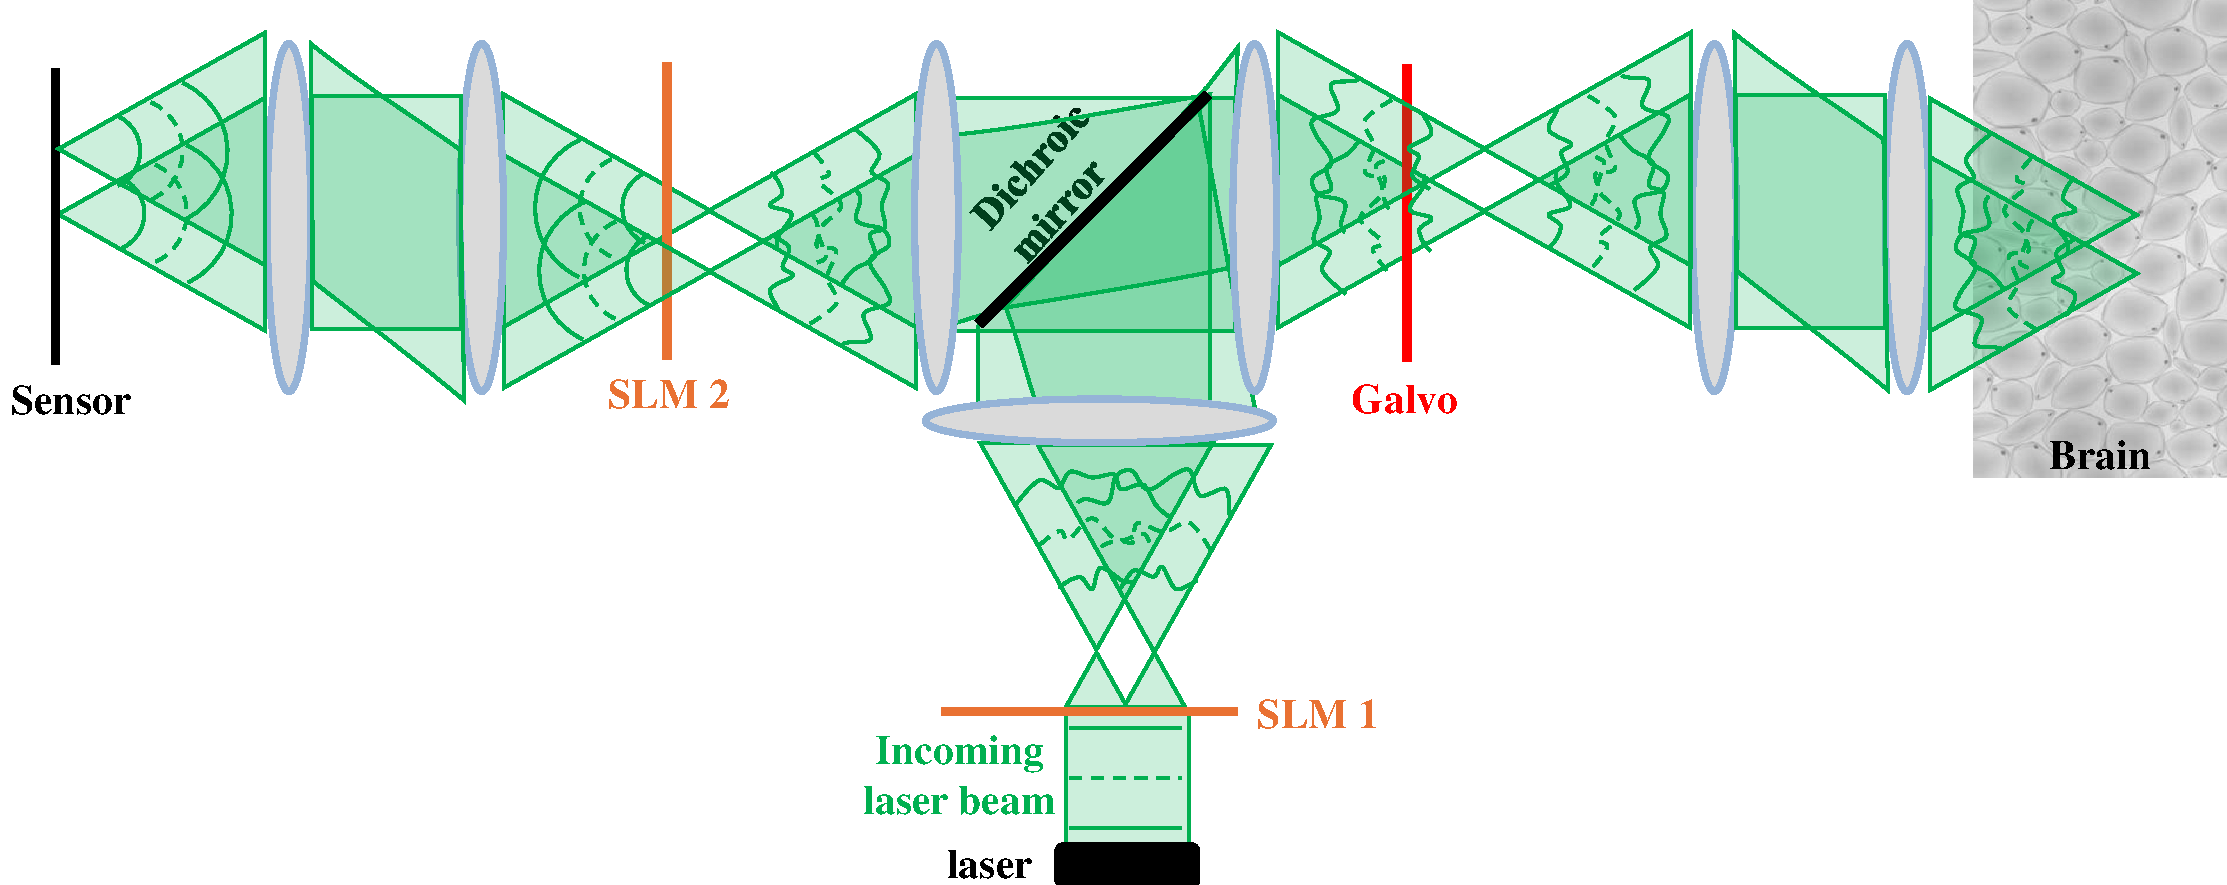
\includegraphics[width= 0.8\textwidth]{figs/system/twoP.pdf}
		%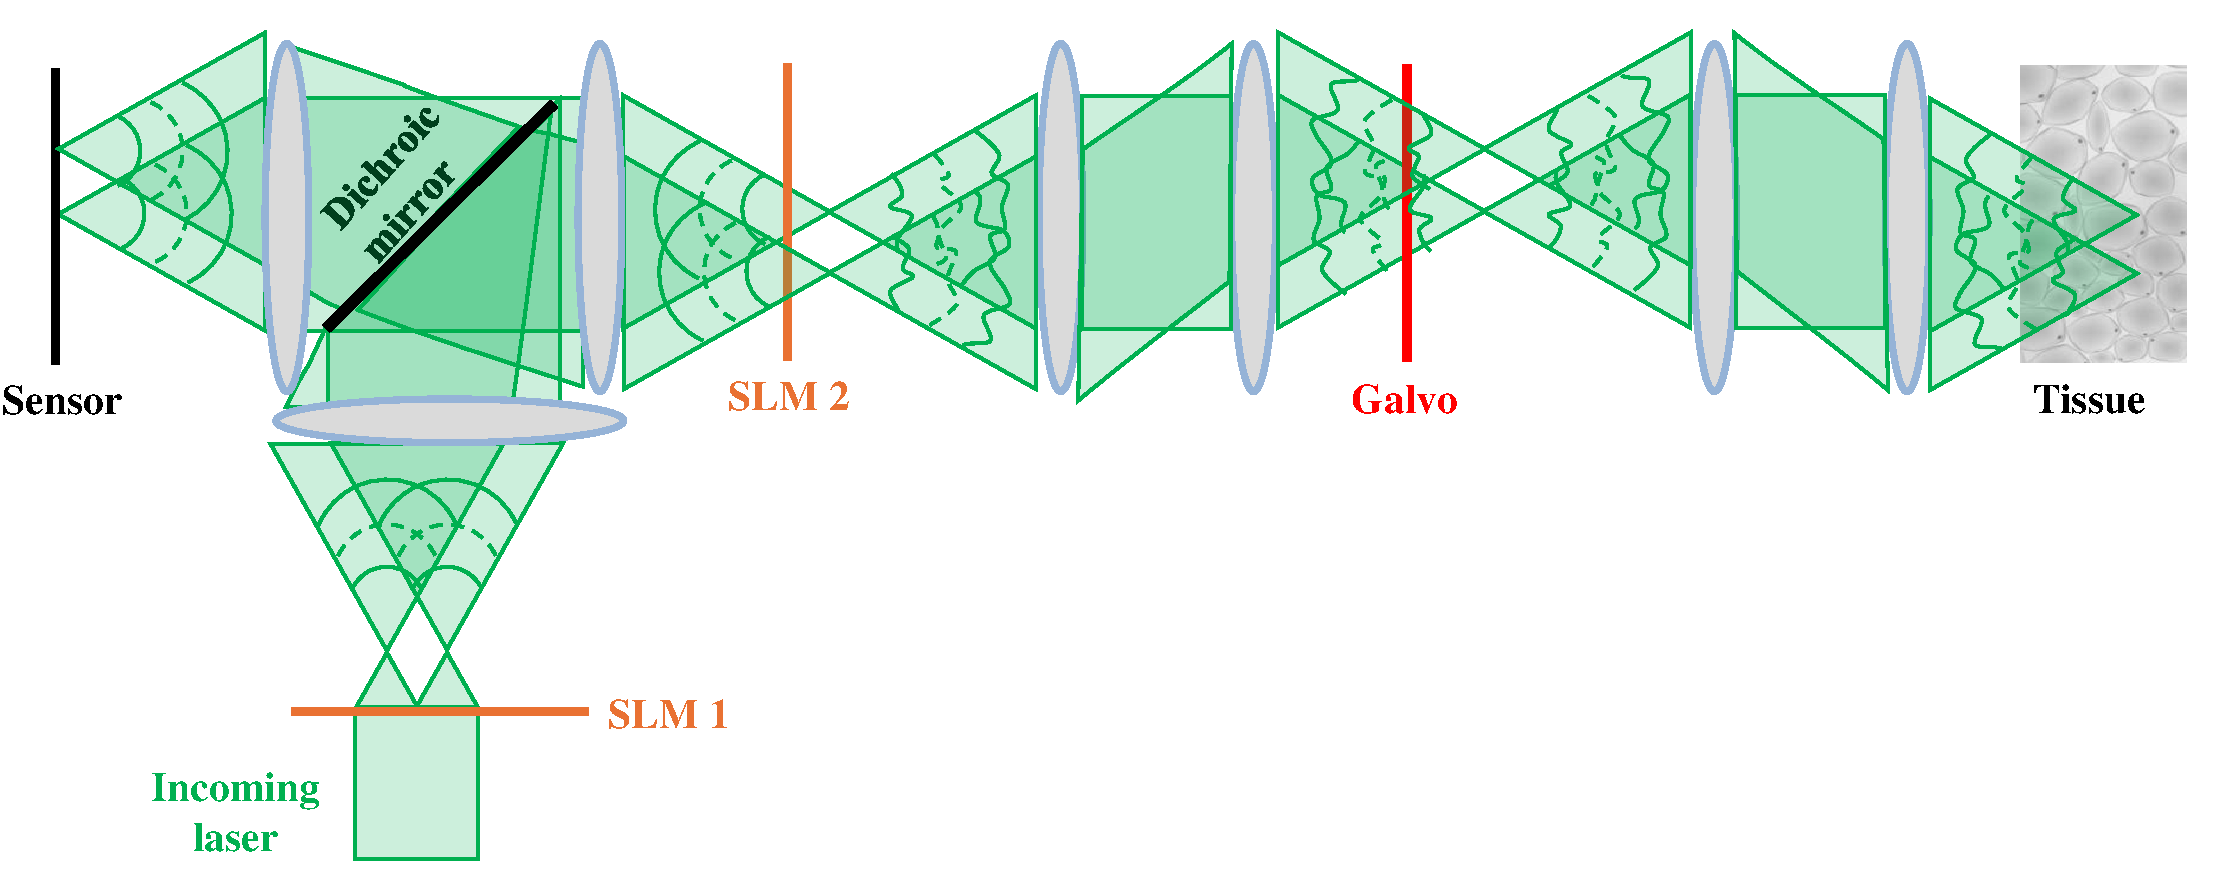
\includegraphics[width= 0.48\textwidth]{figs/system/oneP.pdf}\\
		%(a) Two photon&(b) One photon
		\end{tabular}
	\end{center}
	\caption{{\bf{Wavefront-shaping setup:}} SLM1 generates a hologram directing excitation light to different target neurons, this hologram can also reshape the light to account for tissue aberration. The emitted light is collected via the same objective but directed toward a sensor via a dichroic mirror. The aberration of these wavefronts are corrected at SLM2. The figure illustrates two target neurons at different positions, which are mapped using different SLM pixels. The setup also includes a galvo, which is aimed to scan a diffraction limited illumination point over the neuron area.  } 
%	\caption{{\bf{Wavefront-shaping setup:}}(a) 2P setup: SLM1 generates a hologram directing excitation light to different target neurons, this hologram can also reshape the light to account for tissue aberration. The emitted light is collected via the same objective but directed toward a sensor via a dichroic mirror. The aberration of these wavefronts are corrected at SLM2. The figure illustrates two target neurons at different positions, which are mapped using different SLM pixels. The setup also includes a galvo, which is aimed to scan a diffraction limited illumination point over the neuron area. (b) 1P setup: As the excitation and emission wavefront are similar, they require the same correction pattern, and thus are both modulated at SLM2. In this setup SLM1 is only used to generate two diffraction limited points at the positions of the target neurons.  } 
\label{fig:setup}
\end{figure*}


\subsubsection{Imaging system}
Figure \ref{fig:setup} illustrates our optical setup. To simplify the schematic, we depict SLMs and galvo mirrors as transmitting rather than reflecting surfaces. Excitation light passes through SLM1 to generate a sparse hologram that illuminates the target neurons. The pattern on this SLM can also account for tissue aberrations. To maximize 2P excitation, we design our target points to be diffraction-limited rather than generating a $10\mu m$ spot that can simultaneously excite the entire area of the neuron. We scan the target point over the neuron area using a fast galvo, which is placed in a relay system between the SLM and the tissue. The ideal positioning of this galvo is discussed below. We emphasis that this galvo is used for a very localized scanning over the area of one neuron, not for scanning the entire brain, thus scanning speed should not be a limiting factor. 

While the use of such a galvo is common practice in 2P imaging~\cite{}\Anat{need refs}, 
a key feature of our design is that the same galvo is also used to scan the emitted light. This aligns wavefronts from different points on the neuron onto the same pixels of both the SLM and the sensor.
This alignment is necessary because, to maximize SNR, our goal is to collect the photons emerging from different points on the neuron in the same sensor pixel. For that, the first step is shifting the wavefronts emerging from different excitation points so they are registered on the sensor.
Second, to further maximize SNR, the emitted photons are not only shifted by the galvo but also pass through a second SLM in the emission arm. The goal of this SLM is to reshape the wavefront emitted from a diffraction-limited fluorescent spot inside the volume and focus it into a diffraction-limited spot on the sensor plane. For the brain depths we target, there is sufficient memory effect correlation~\cite{osnabrugge2017generalized,SeeThroughSubmission} between wavefronts emitted from points in a small local area of $10\mu m$, allowing us to correct all of them with the same SLM pattern. Another important property we aim to utilize is that for such brain depths, the speckle from a single spot has a medium size aberration, whose diameter is usually a few dozen pixels wide. Therefore, the wavefronts resulting from different neurons can be corrected by separate SLM pixels.
We emphasis that if the support of the aberration is a few dozen pixel wide it can still cover hundreds of even thousands of SLM pixels, providing a significant number of correction modes, far beyond the low order aberrations of adaptive optics systems. 

We note that 2P excitation is usually combined with temporal focusing to further enhance depth sectioning~\cite{hernandez2016three,sun2018four,pegard2017three,mardinly2018precise,sridharan2021high}. This idea is a simple addition to our system, but for simplicity, we will not discuss it here.



%\boldstart{2P system:} we have one SLM to reshape the incoming beam and generate a sparse hologram to illuminate the target neurons. To maximize the 2P excitation we design our target points to be diffraction limited rather than generate a $10\mu m$ spot that can simultaneously excite the full area of the neuron. We scan the target point over the neuron area using a fast galvo, which is placed in a relay system between the SLM and the tissue. We discuss the ideal positioning of this galvo below.
%While the usage of such a galvo is a common practice in 2P imaging~\cite{}\Anat{need refs}, the new part of our design is that the same galvo is used to scan the outgoing light so that wavefronts emerging from different points on the neuron are aligned to the same pixels on the SLM/sensor allowing us to image a diffraction limited pattern. To maximize SNR our goal is to collect the photons emerging from different points on the neuron in the same sensor pixel. For that, the first step is shifting the wavefronts so they are registered.
%To maximize SNR the emitted photons are not only shifted by the galvo, but also pass through a second SLM in the emission arm. The goal of this SLM is to reshape the wavefront emitted from a diffraction limited fluorescent spot inside the volume  and focus it into a diffraction limited spot on the sensor plane. 
%We explain below that for the brain depths we target here, there is sufficient memory effect correlation~\cite{} between wavefronts emitted from points in a small local area of $10\mu m$ and we can correct all of them with the same SLM pattern.
%Another important property we aim to utilize is that for such brain depths the speckle from a single spot has a modest aberration, whose support is limited to only spread over a few dozen pixels. Therefore, the wavefronts resulting from different neurons  can be corrected by separate SLM pixels. 
%
%We  note that usually this 2P excitation is combined with temporal focusing to further enhance depth sectioning. This idea is orthogonal to the proposed correction and for simplicity we will not discuss it here. 

For a 1P correction, we can utilize the same setup. Given the proximity of the excitation and emission wavelengths, we can employ the same SLM pattern to reshape both. In practice, system alignment becomes significantly simpler if we not only use the same pattern but also pass both incoming and outgoing wavefronts through the same physical SLM. Consequently, we can reposition the dichroic mirror to be placed after SLM2.


%\boldstart{1P system:} Is similar to the 2P  system with one impotent difference. Even for modest tissue depths the excitation light is also aberrated, and we need to use the SLM to reshape the incoming light as well. Since the excitation and emission wavelengths are very close, we use the {\em same SLM pattern } to reshape both. The system alignment is significantly simpler if we not only use the same pattern, but actually pass both incoming and outgoing wavefronts via the same physical SLM. 
%Before the wavefront shaping SLM the excitation arm includes another SLM whose task is to create a sparse set of points in the target neural positions. Since in a 1P system the laser power does not pose  major limits we can also use a binary DMD as in~\cite{} which blocks light rather than redistribute it. 

We plan to use an SLM technology recently developed by Taxes Instrument~\cite{PLM-TI_2019}, featuring $800 \times 1358$ pixels. The advantages of this SLM include its use of mirrors instead of liquid crystals, making it not polarization sensitive. Additionally, it supports a fast refresh rate of $1.4$ kHz.




To measure voltage activity, we need to image neurons at kilohertz frame rates. Although fast reading from a wide field of view sensor is challenging, we can significantly increase the frame rate by reducing the number of rows we read. Many modern sensors can easily read a few dozen rows at a 2 kHz frame rate. By incorporating the SLM, we can tilt the images of all target neurons into a small number of sensor rows and read them at a higher frame rate.
For 2P imaging, where the number of target neurons is limited, we can replace the 2D sensor with a sparse array of PMT detectors and use the SLM to direct light to these detectors. This approach will allow us to increase the frame rate by orders of magnitude.




\subsubsection{Correction algorithms}
\boldstart{2P emission correction:} At modest tissue depths, a 2P excitation beam propagates with minimal aberration. Since the emission is proportional to the square of the excitation power, the emitted light primarily returns from a single point guide-star. To correct aberration, we need to measure the complex wavefront emerging from the guide-star and apply its conjugate on the SLM.
There are various wavefront measurement strategies available, with the simplest being the use of a Shack-Hartmann wavefront sensor~\cite{Platt2001HistoryAP,Aviles-Espinosa:11,Cha2010SHwavefrontsensor}. Alternatively, the wavefront can be estimated using a  phase retrieval optimization problem~\cite{candes2015}, e.g. using phase diversity~\cite{Dean2003,Robert1982}, or a random perturbation scheme~\cite{WISH2019}.
To achieve this, we display a small number of $3-5$ known modulation patterns on the SLM, measure the intensity of the resulting aberrated speckle pattern, and solve an optimization problem to determine the complex phase of the wavefront.

\boldstart{2P excitation correction:}
To correct the excitation arm, we adhere to the fundamental principle of 2P excitation, which states that focusing more energy into a single point increases the emitted power. Mathematically, if $I(\ptd)$ represents the excitation laser power at point 
$\ptd$ in the volume, the emitted power is proportional to the square of the excitation, integrated throughout the volume:
\BE\label{eq:emitted-power-2P}
\int_r |I(\ptd)|^2.
\EE
At the same time, a wavefront shaping modulation can only alter the phase of the wavefront, not increase the laser power. Therefore, it can only redistribute the energy within the volume. For any planar segment in the volume, the excitation energy is bounded by a constant $C$ proportional to the laser power:
\BE
\int_\ptd |I(\ptd)|\leq C.
\EE 
Under this constraint, it is evident that the emitted energy in the equation above is maximized if $I(\ptd)$ is an impulse, meaning we need to find a wavefront shaping modulation that focuses as much energy as possible into a single point.
Based on this observation, algorithms in the wavefront shaping and adaptive optics literature~\cite{Katz:14,Ji2017review,HampsonBooth21review,Rodriguez2021Adaptive} adjust the SLM parameters to maximize the emitted energy. We will follow a similar strategy in our research.


\boldstart{1P correction:}
Until recently, estimating wavefront shaping modulation using non-invasive 1P feedback was considered a much more challenging problem. Unlike in 2P excitation, where the emitted light is proportional to the square of the excitation (\equref{eq:emitted-power-1P}), in 1P excitation, the emitted light is linearly proportional to the excitation:
\BE\label{eq:emitted-power-1P}
\int_\ptd |I(\ptd)|.
\EE
This means that the amount of emitted energy does not change whether the energy is focused or widely distributed. We recently overcame this challenge~\cite{DrorNatureComm24} by proposing a confocal SLM correction in both the excitation and emission arms. Instead of measuring the total energy emitted from the fluorescent volume, we measure the energy that we can bring into a single sensor pixel. If we find a modulation that focuses all the laser energy into a single point in the volume, the same correction can also undo the scattering of the emitted light and bring it all into a single point on the sensor. Mathematically, we can prove that the confocal energy at that pixel is again proportional to the squared intensity, as in the 2P case:
\BE\label{eq:emitted-power-1P-conf}
\int_\ptd |I(\ptd)|^2.
\EE
Therefore, in our recent work~\cite{DrorNatureComm24}, we adjust the SLM parameters to maximize the confocal energy, demonstrating that such modulations also focus the light into a single point inside the tissue volume. This approach provides a simple, non-invasive method to achieve effective wavefront shaping modulations using inexpensive 1P feedback. Additionally, correcting both the incoming and outgoing light significantly increases the noise robustness of our approach, allowing it to work with a lower photon count. We also developed algorithms for rapid modulation estimation using an optical implementation of the gradient descent algorithm~\cite{monin2025rapidwavefrontshapingusing}. As part of this project we aim to further develop  algorithmic tools to help accelerating the modulation estimation and improving its noise robustness.

	\begin{figure*}[t!]
	\begin{center}
		
		\begin{tabular}{@{}c@{~~}c@{~~}c@{~~~~}|@{~~~~}c@{}c@{~~}c@{}c@{~~}c@{}c@{}}
			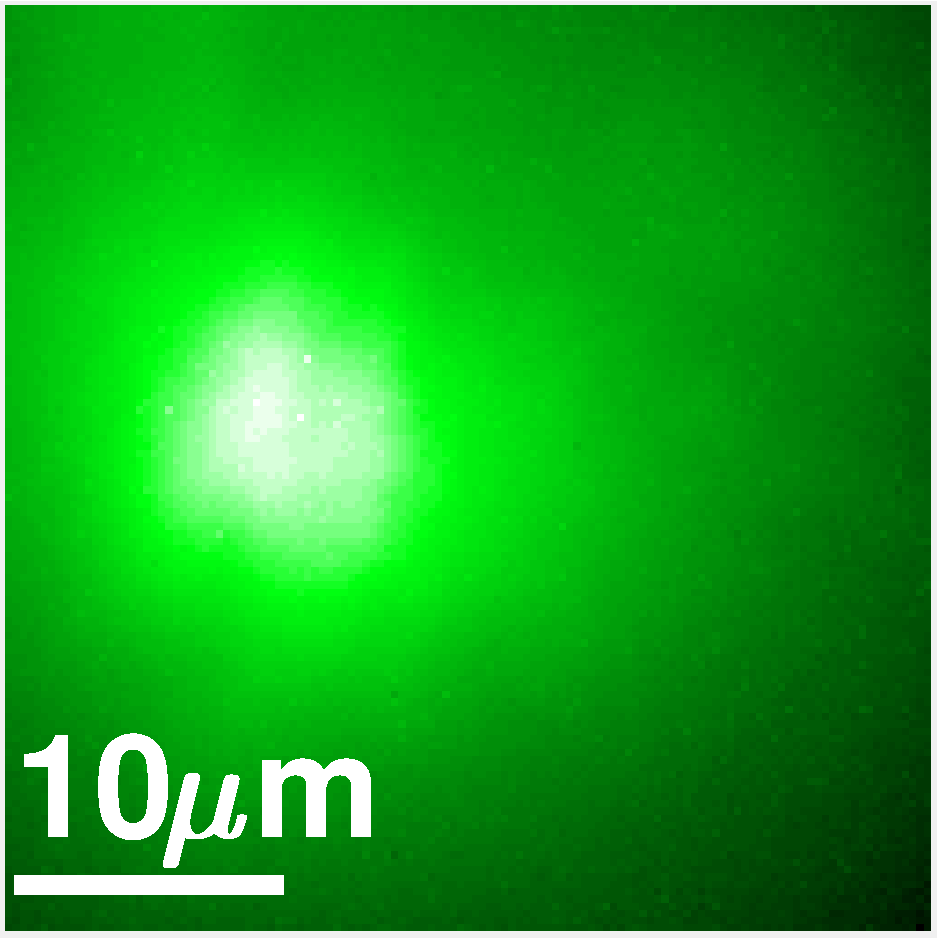
\includegraphics[width= 0.13\textwidth]{figs/confocal_res/fig_big_area/2023_06_08_18_48_03/1.pdf}&
			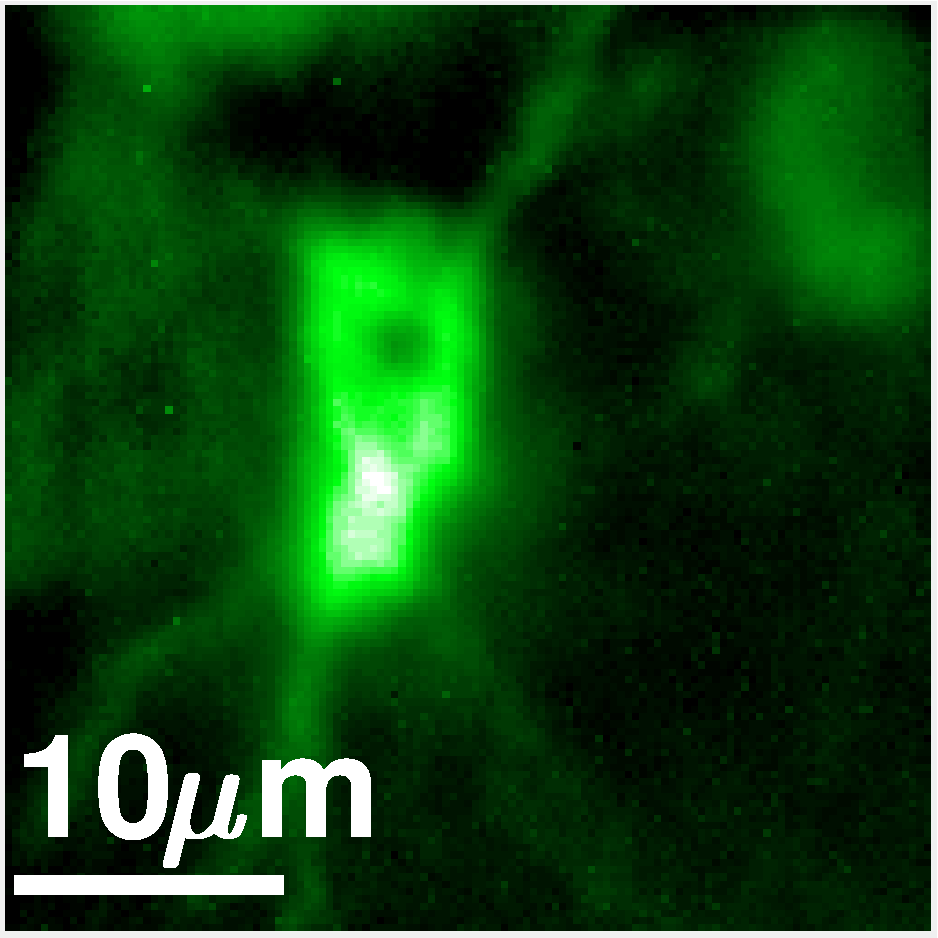
\includegraphics[width= 0.13\textwidth]{figs/confocal_res/fig_big_area/2023_06_08_18_48_03/2.pdf}&
			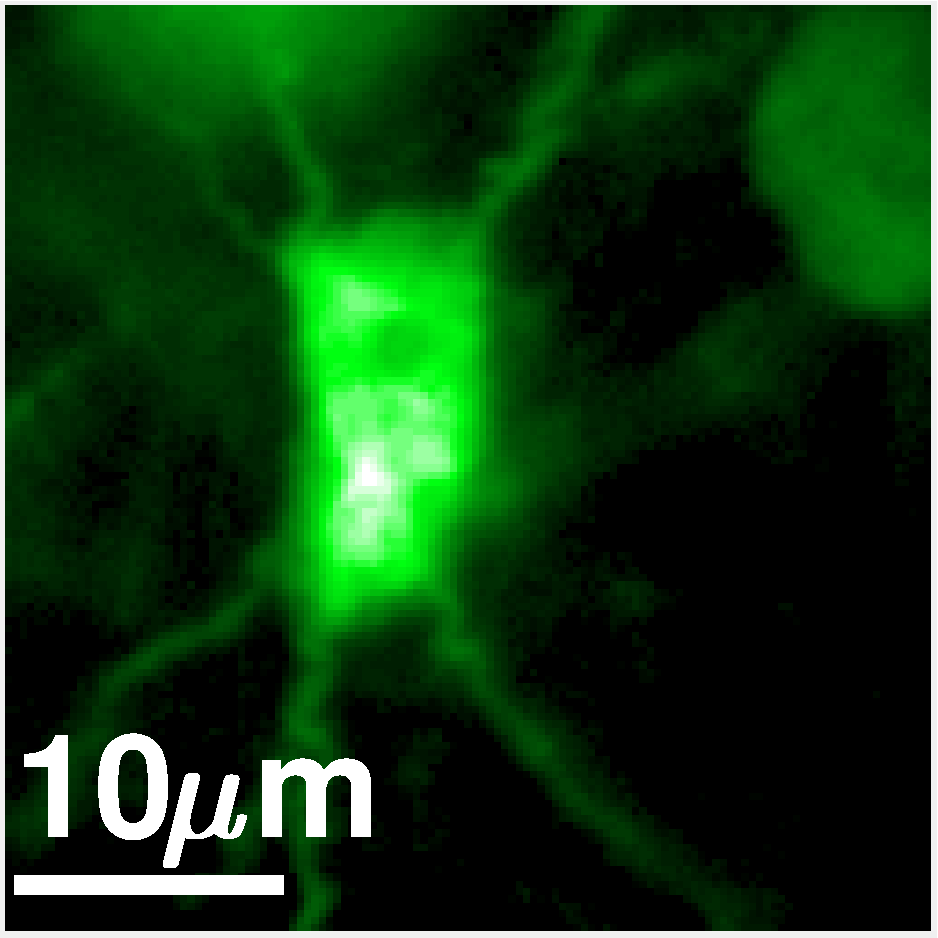
\includegraphics[width= 0.13\textwidth]{figs/confocal_res/fig_big_area/2023_06_08_18_48_03/3.pdf}&
		
			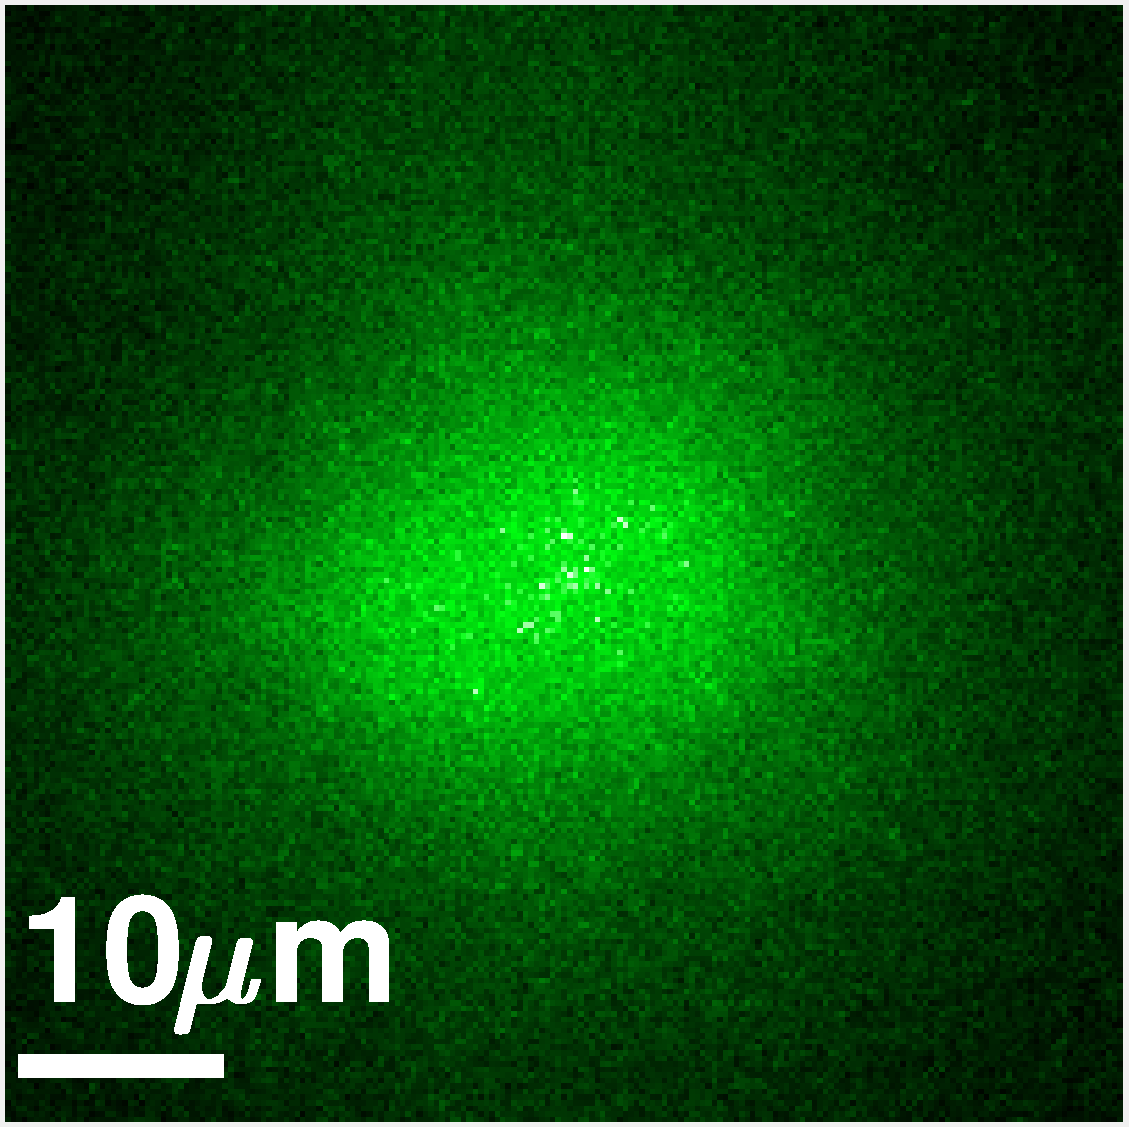
\includegraphics[width = 0.13\textwidth]{figs/confocal_res/fig_converging/2023_01_11_18_28_55/BSI_init.pdf}&
			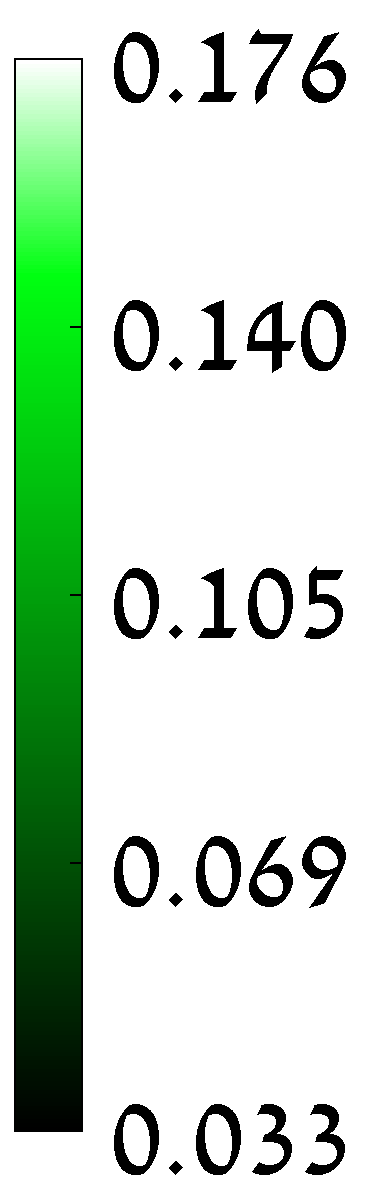
\includegraphics[height = 0.13\textwidth]{figs/confocal_res/fig_converging/2023_01_11_18_28_55/BSI_init_colorbar.pdf}&
			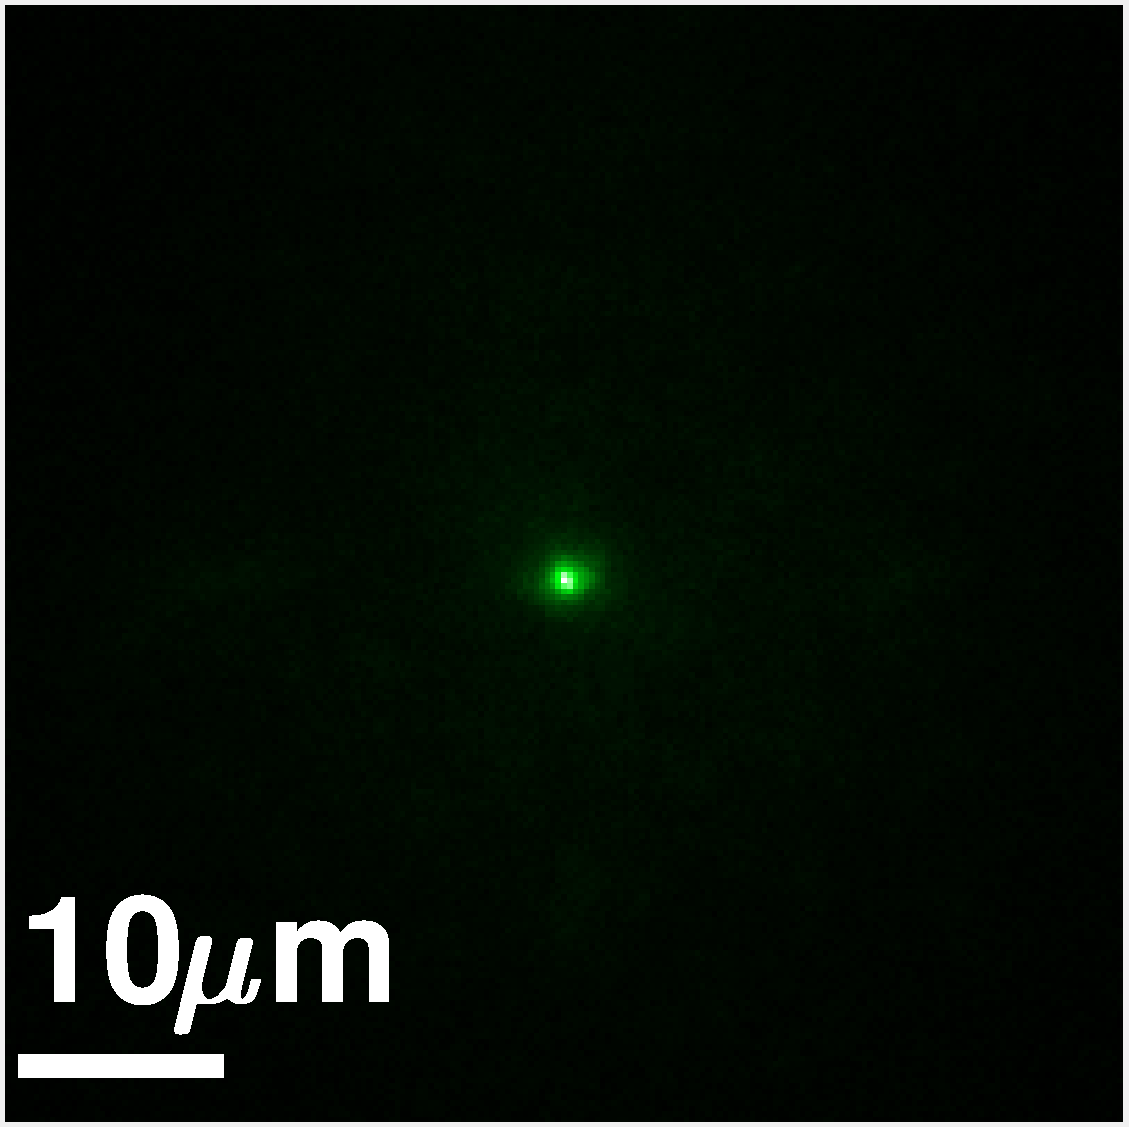
\includegraphics[width = 0.13\textwidth]{figs/confocal_res/fig_converging/2023_01_11_18_28_55/BSI_fin.pdf}&
			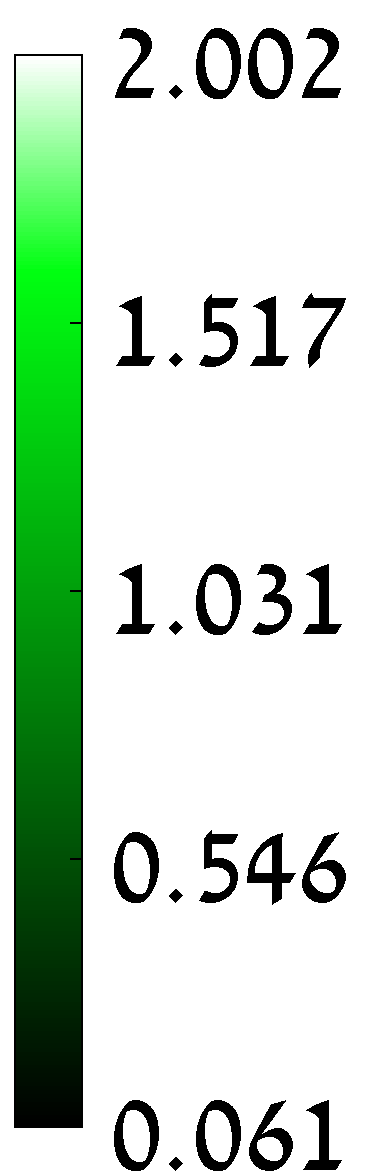
\includegraphics[height = 0.13\textwidth]{figs/confocal_res/fig_converging/2023_01_11_18_28_55/BSI_fin_colorbar.pdf}&
			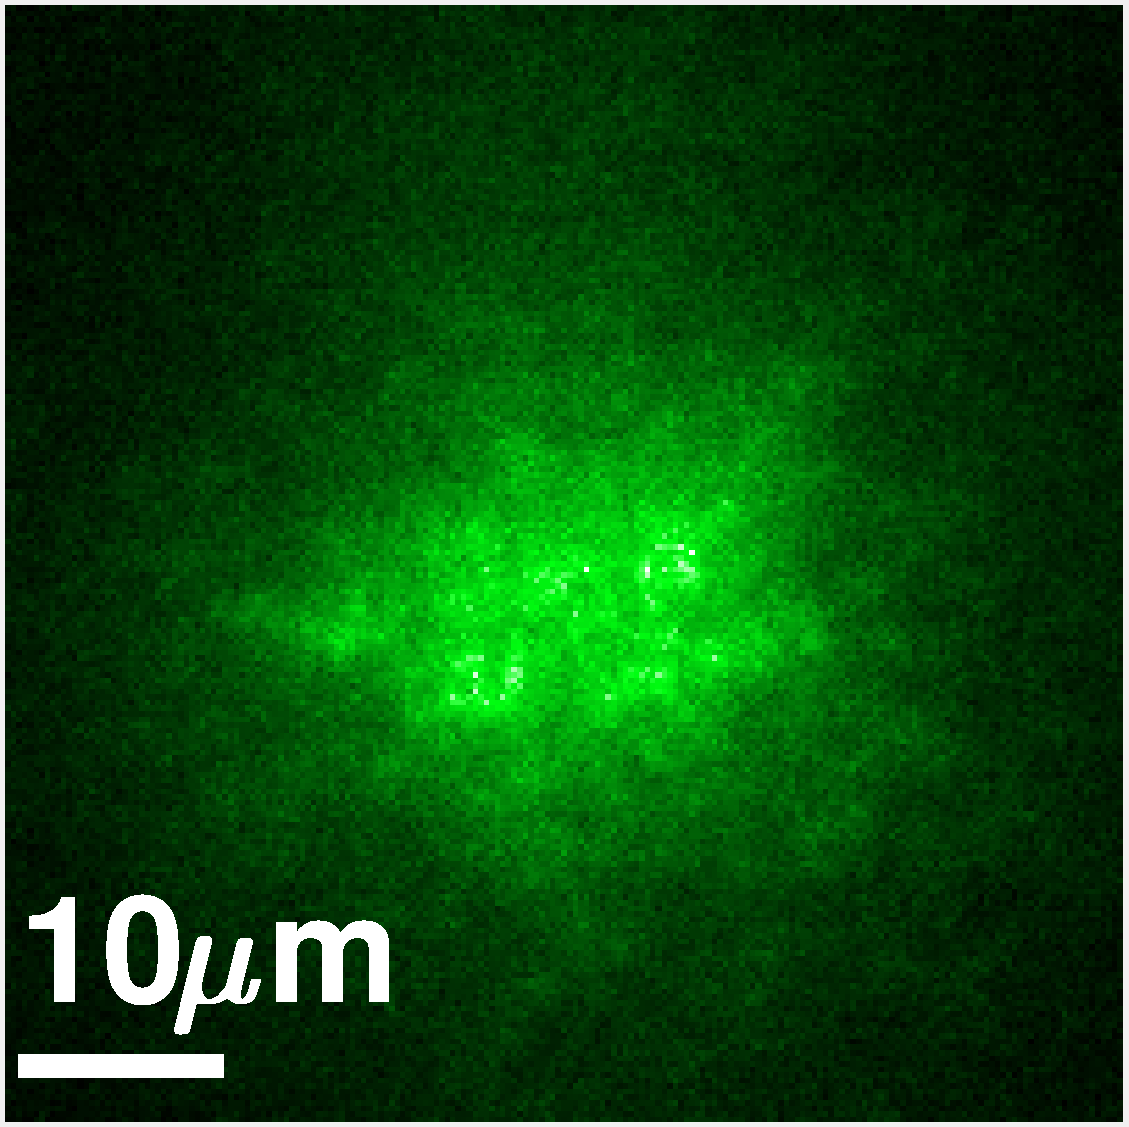
\includegraphics[width = 0.13\textwidth]{figs/confocal_res/fig_converging/2023_01_11_18_28_55/BSI_fin_psf.pdf}&
			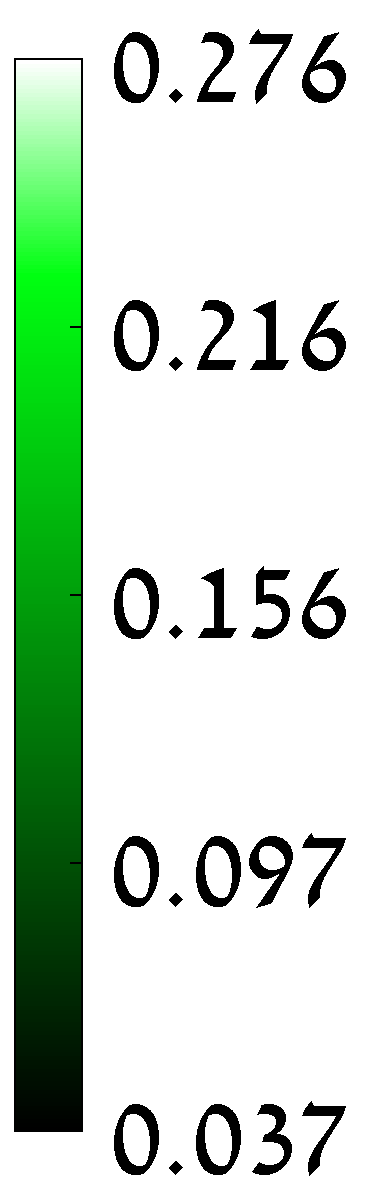
\includegraphics[height = 0.13\textwidth]{figs/confocal_res/fig_converging/2023_01_11_18_28_55/BSI_fin_psf_colorbar.pdf}\\
			
			
			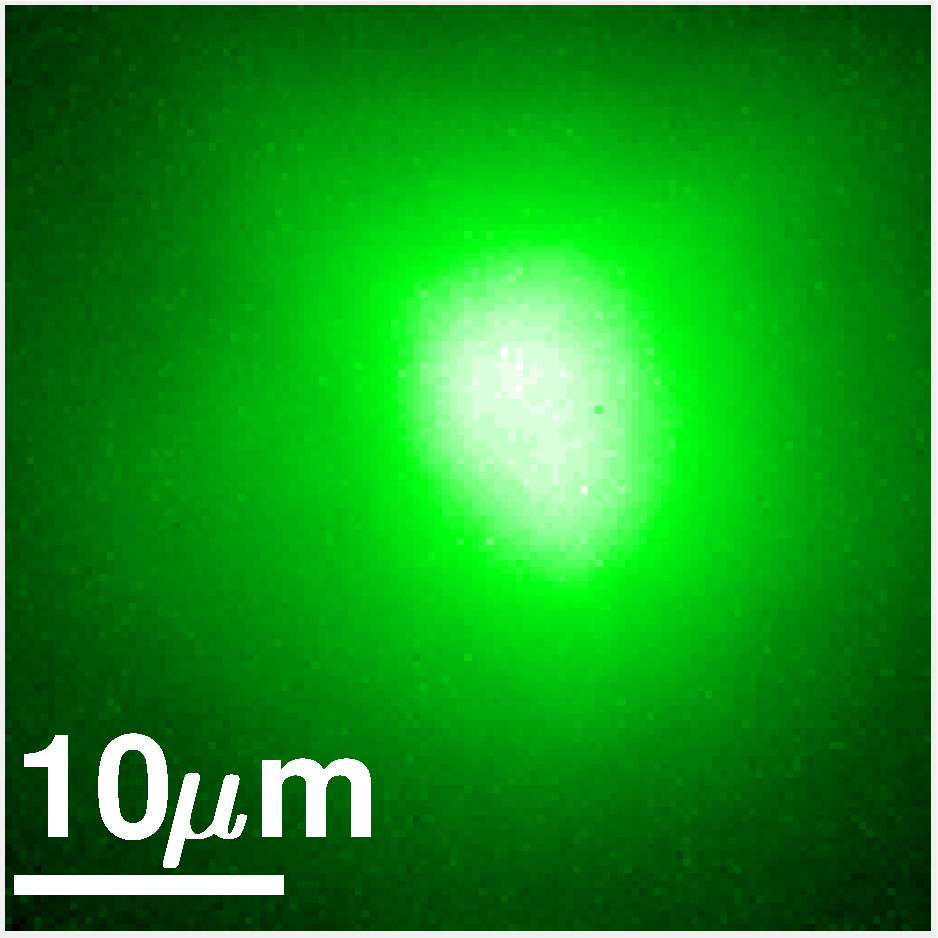
\includegraphics[width= 0.13\textwidth]{figs/confocal_res/fig_big_area/2023_06_05_15_57_55/1.pdf}&
	    	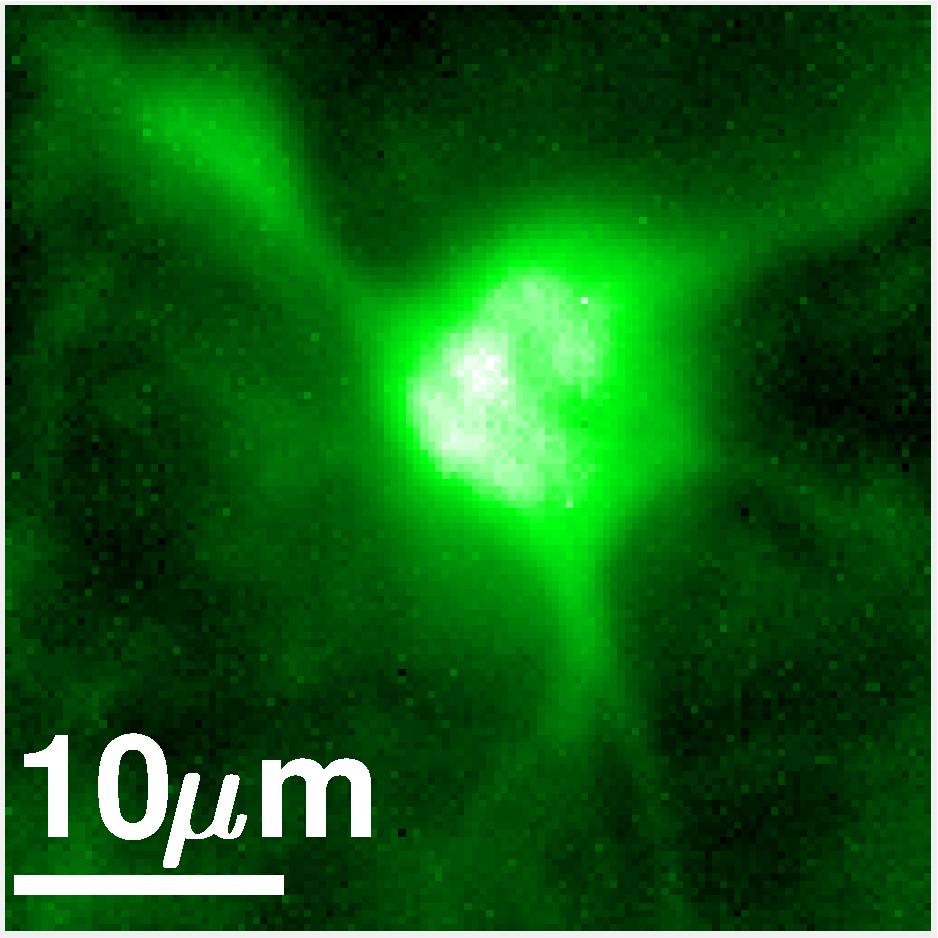
\includegraphics[width= 0.13\textwidth]{figs/confocal_res/fig_big_area/2023_06_05_15_57_55/2.pdf}&
	    	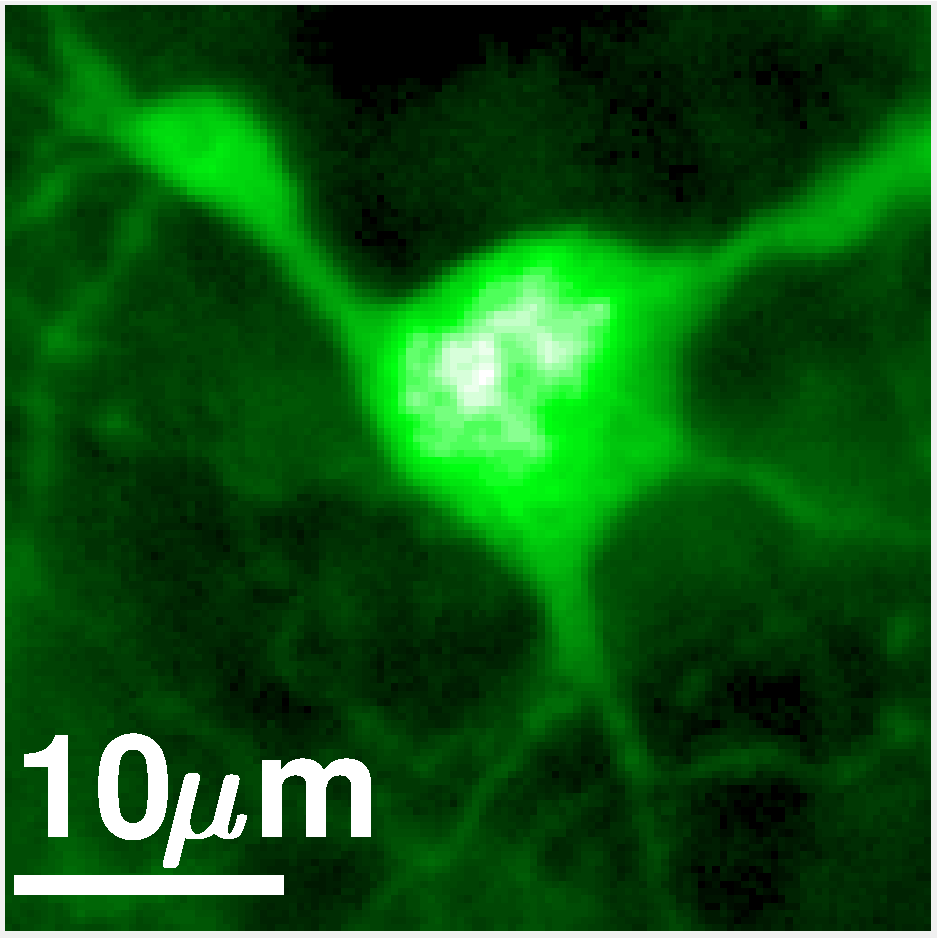
\includegraphics[width= 0.13\textwidth]{figs/confocal_res/fig_big_area/2023_06_05_15_57_55/3.pdf}&
		
			
			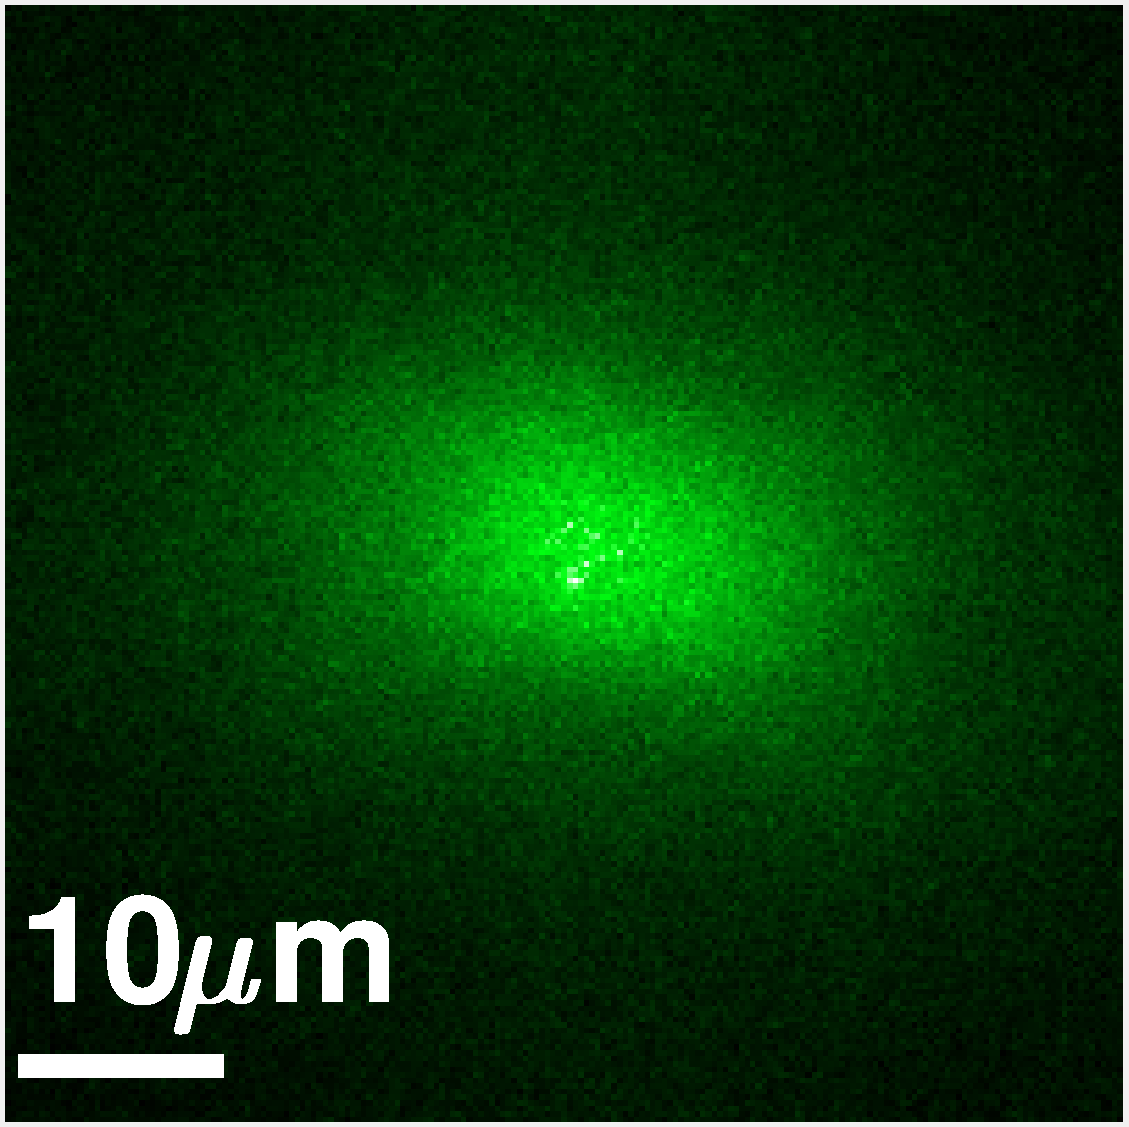
\includegraphics[width = 0.13\textwidth]{figs/confocal_res/fig_converging/2023_01_10_17_18_44/BSI_init.pdf}&
			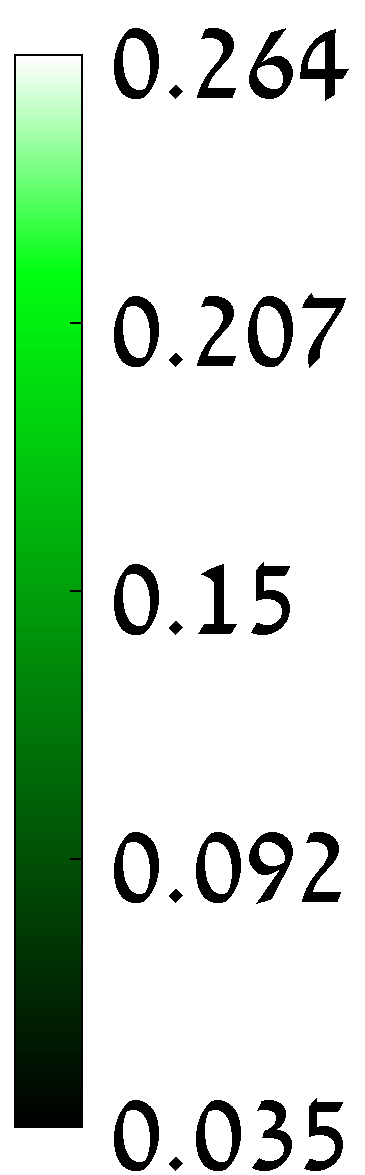
\includegraphics[height = 0.13\textwidth]{figs/confocal_res/fig_converging/2023_01_10_17_18_44/BSI_init_colorbar.pdf}&
			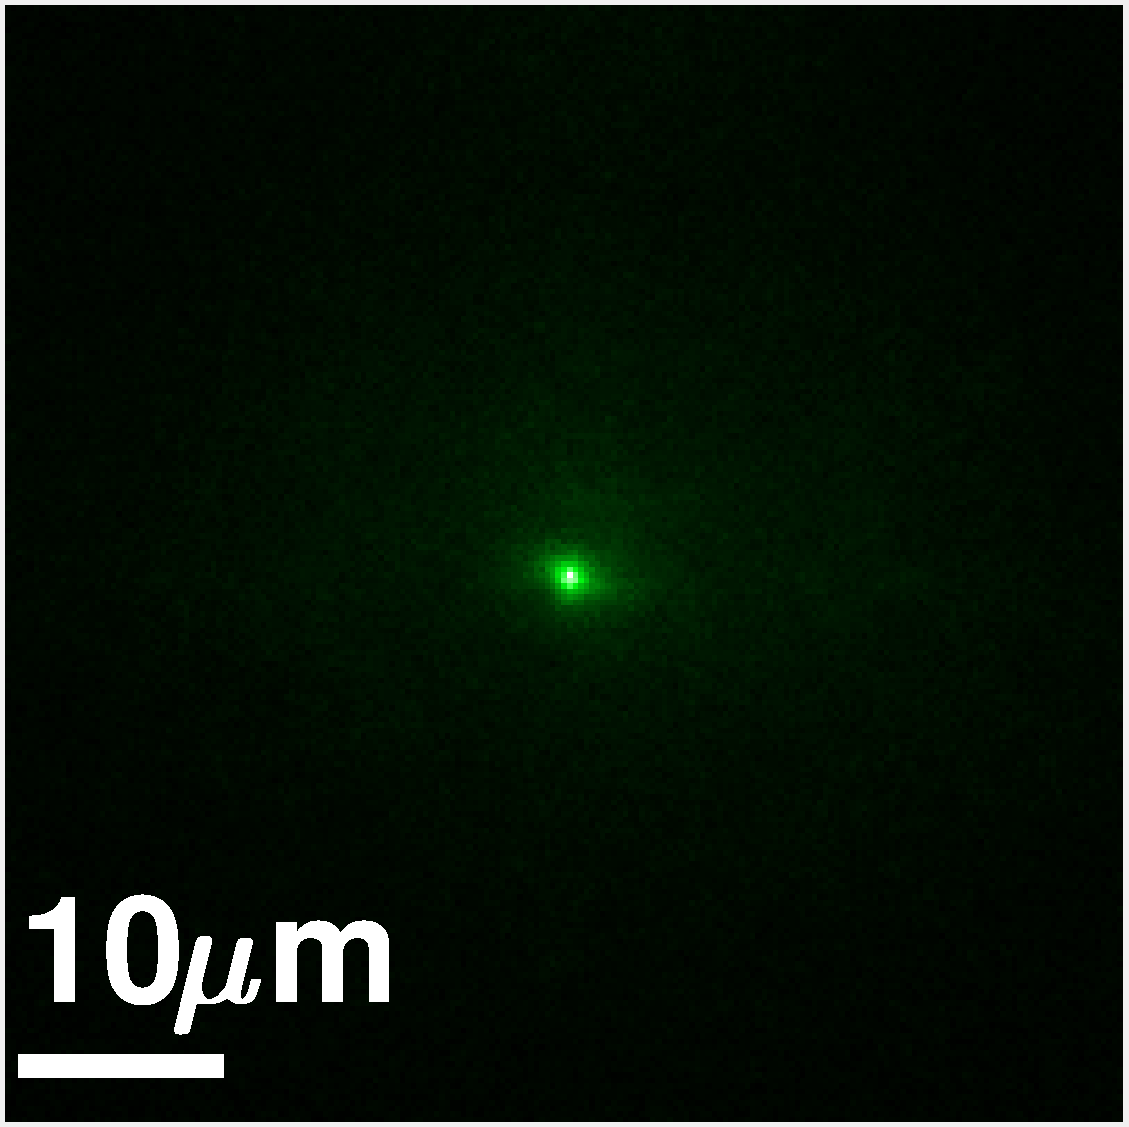
\includegraphics[width = 0.13\textwidth]{figs/confocal_res/fig_converging/2023_01_10_17_18_44/BSI_fin.pdf}&
			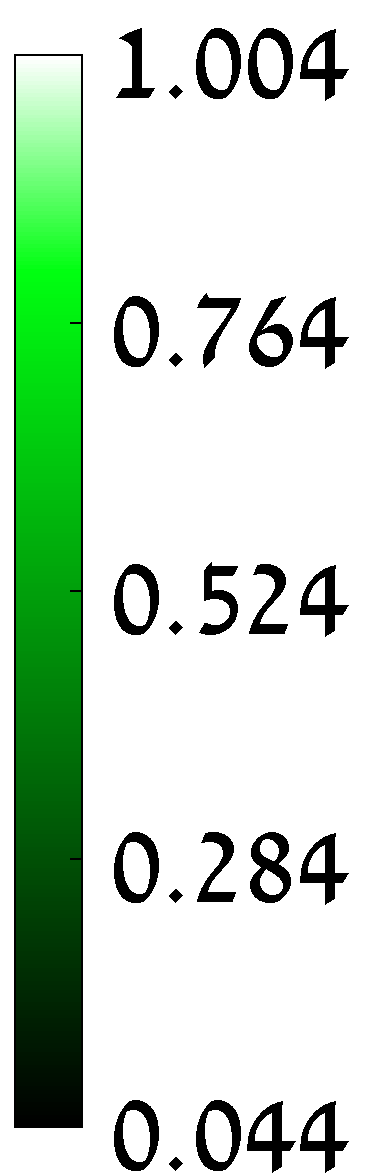
\includegraphics[height = 0.13\textwidth]{figs/confocal_res/fig_converging/2023_01_10_17_18_44/BSI_fin_colorbar.pdf}&
			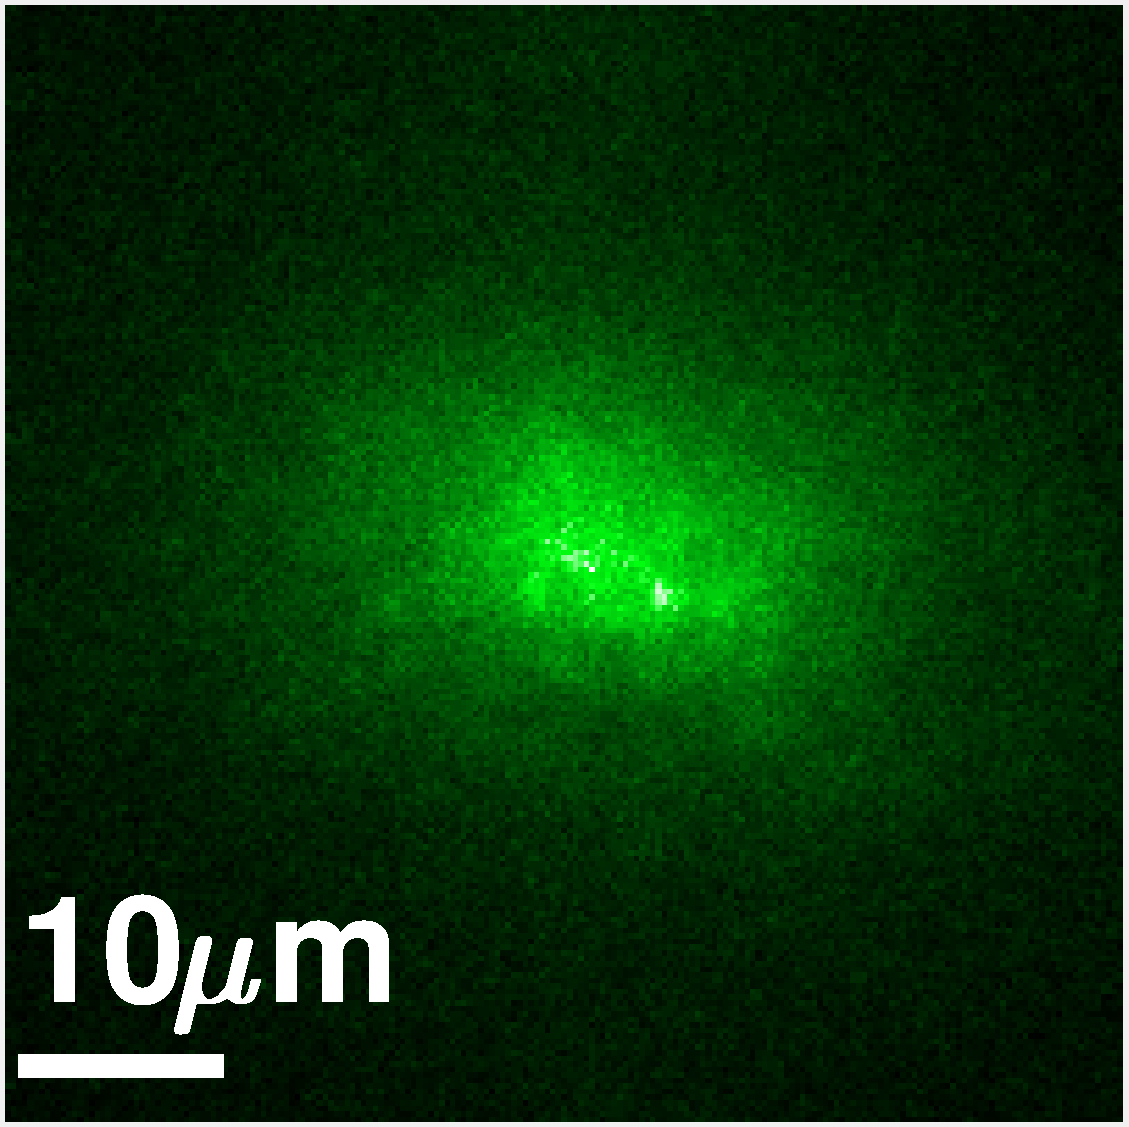
\includegraphics[width = 0.13\textwidth]{figs/confocal_res/fig_converging/2023_01_10_17_18_44/BSI_fin_psf.pdf}&
			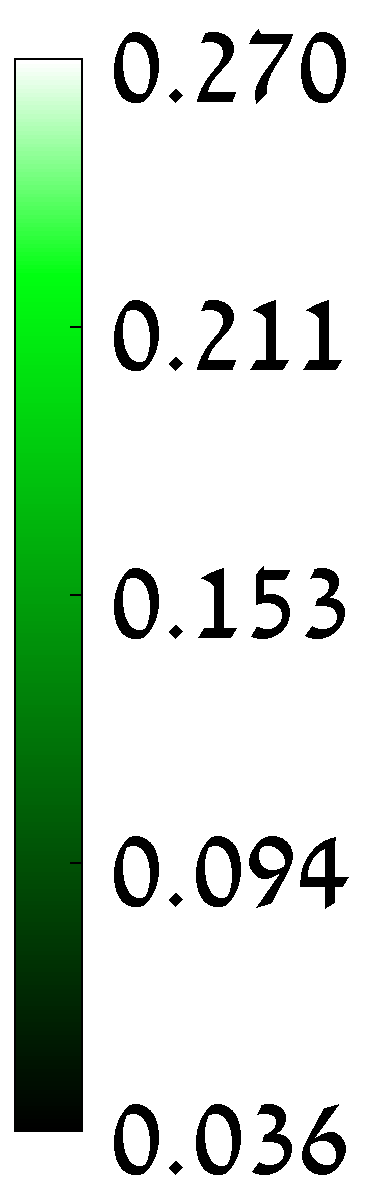
\includegraphics[height = 0.13\textwidth]{figs/confocal_res/fig_converging/2023_01_10_17_18_44/BSI_fin_psf_colorbar.pdf}\\
			
			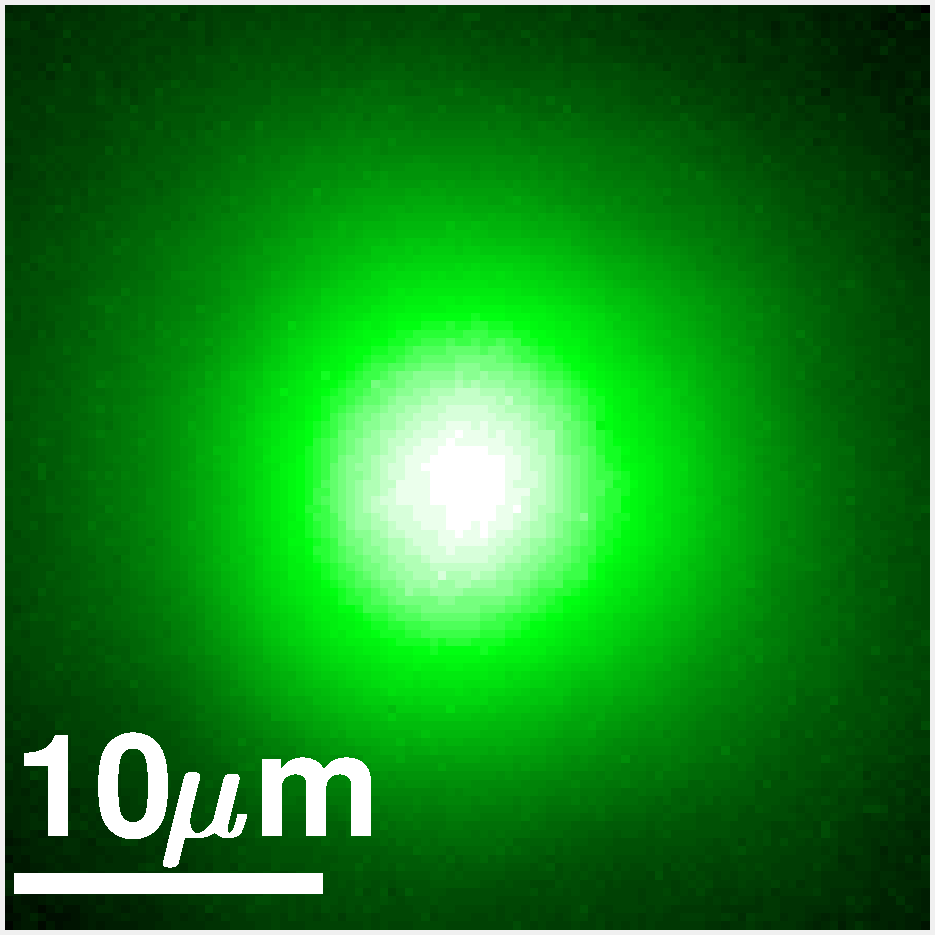
\includegraphics[width= 0.13\textwidth]{figs/confocal_res/fig_big_area/2023_05_16_17_21_45/1.pdf}&
			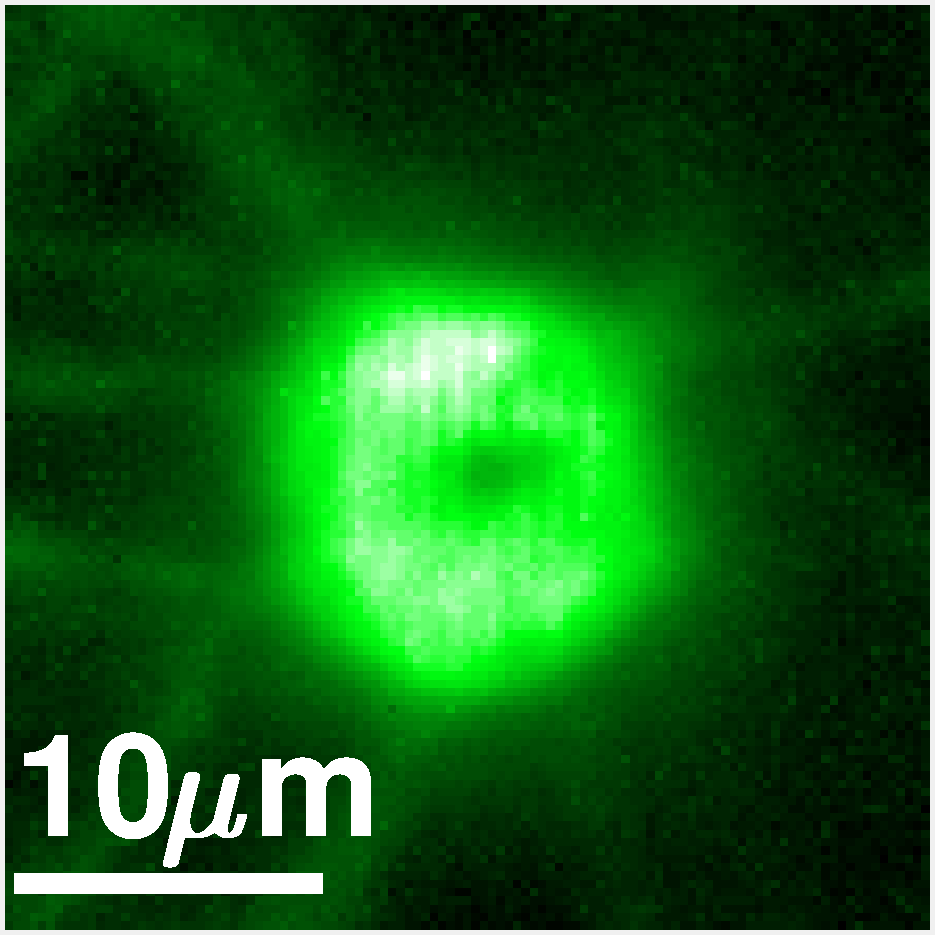
\includegraphics[width= 0.13\textwidth]{figs/confocal_res/fig_big_area/2023_05_16_17_21_45/2.pdf}&
			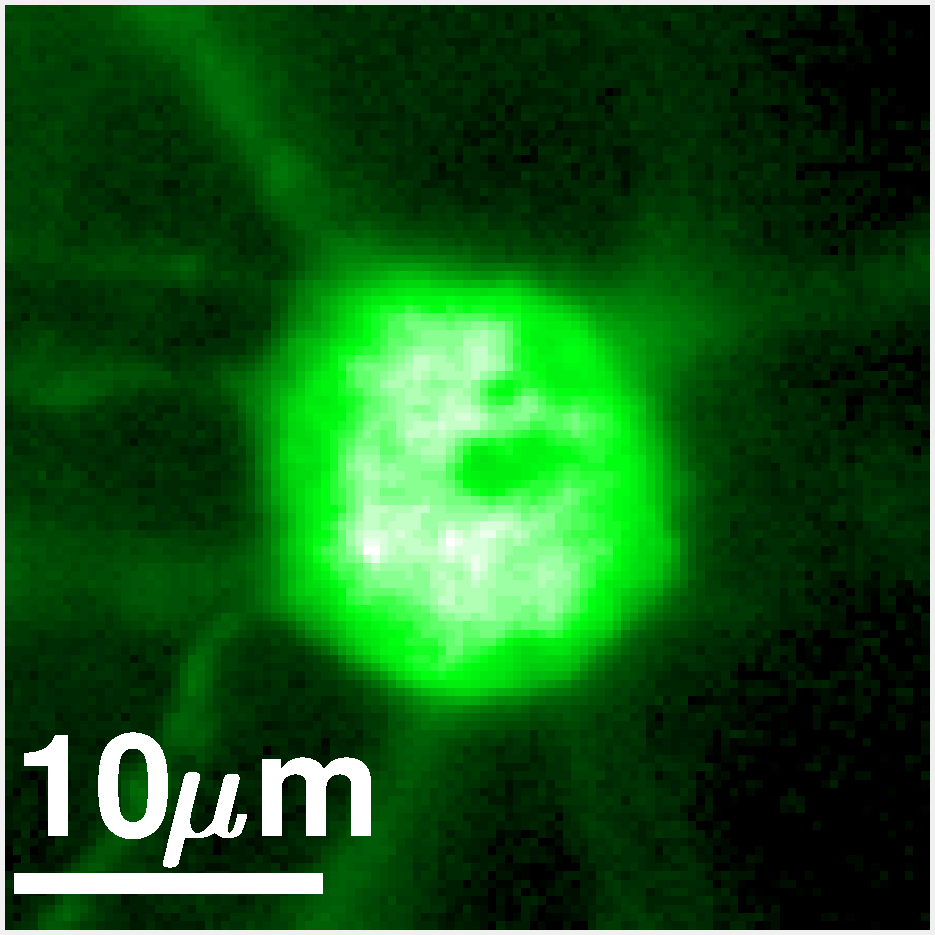
\includegraphics[width= 0.13\textwidth]{figs/confocal_res/fig_big_area/2023_05_16_17_21_45/3.pdf}&
			
				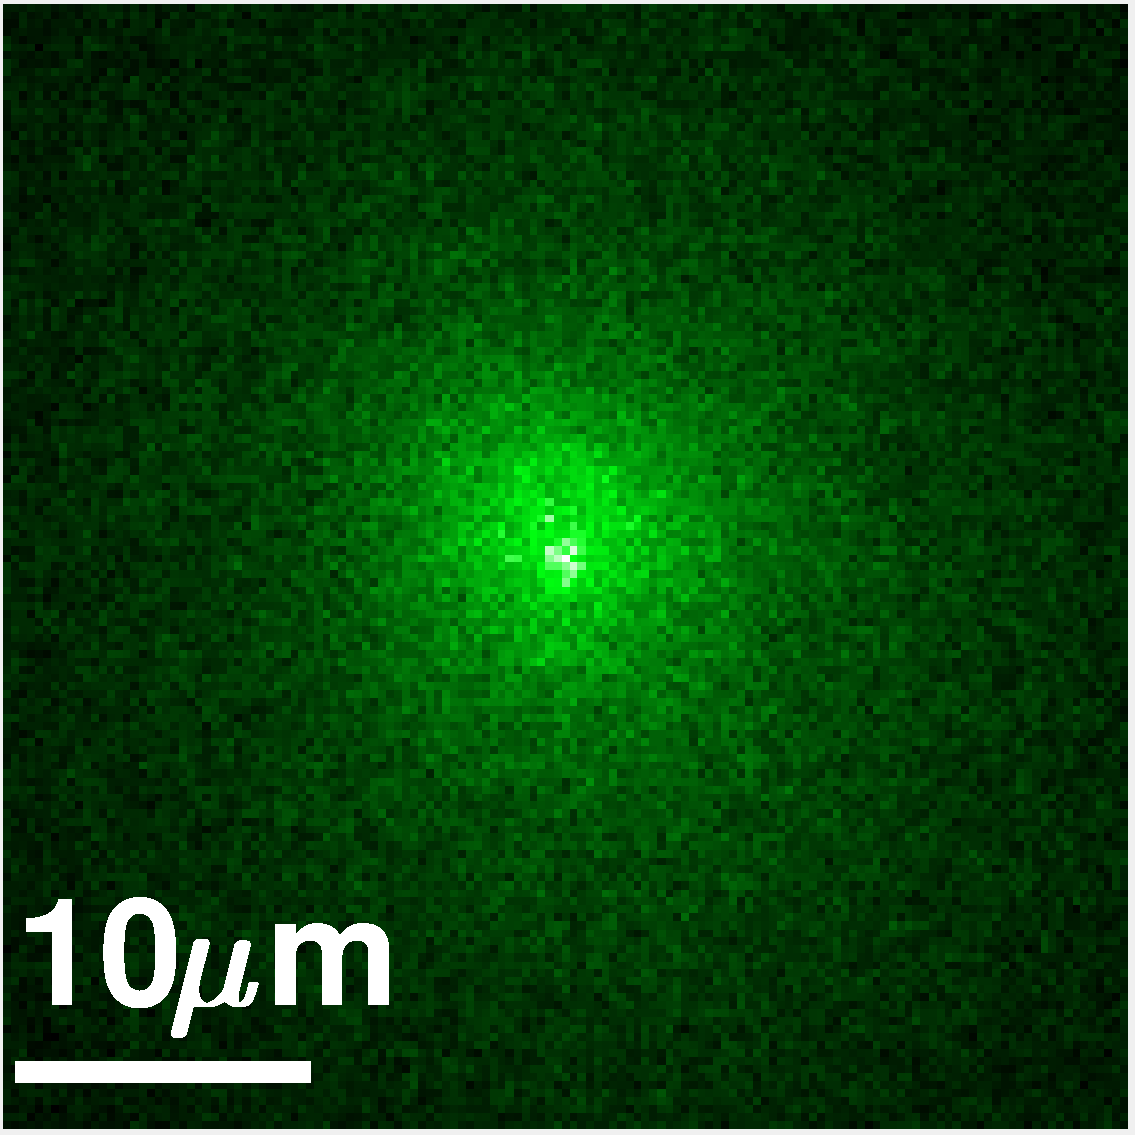
\includegraphics[height = 0.13\textwidth]{figs/confocal_res/fig_converging/4_BSI_init.pdf}&
			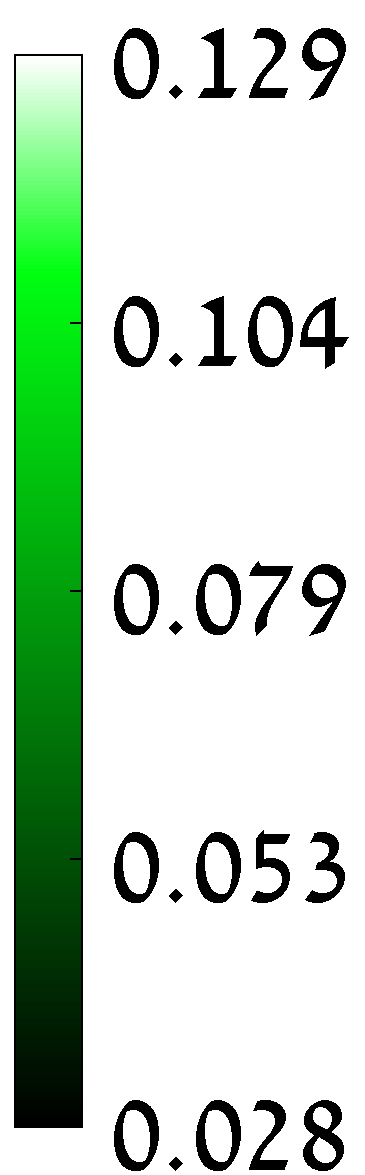
\includegraphics[height = 0.13\textwidth]{figs/confocal_res/fig_converging/4_BSI_init_colorbar.pdf}&
			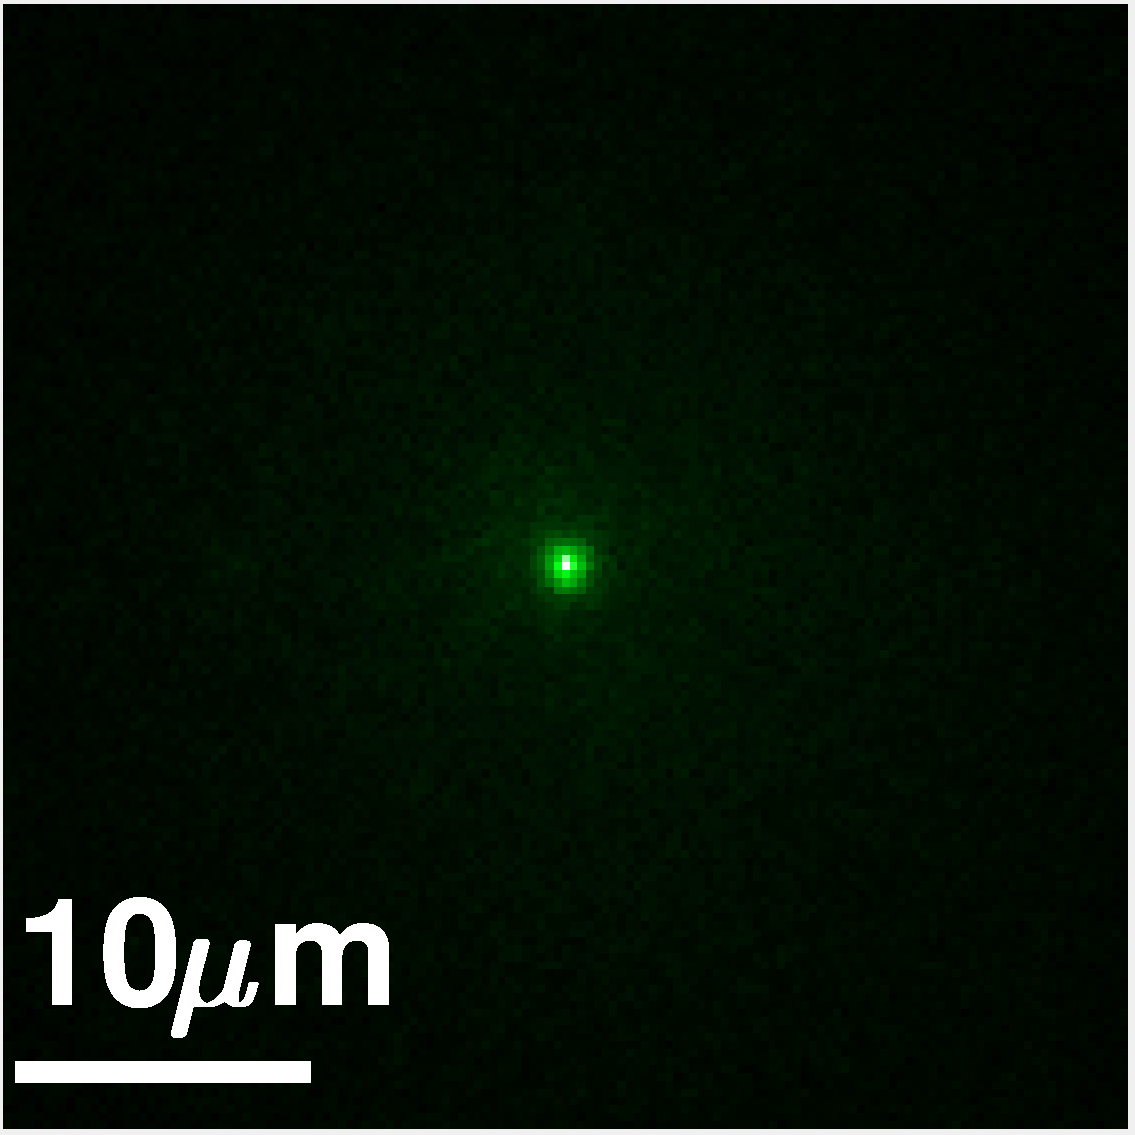
\includegraphics[height = 0.13\textwidth]{figs/confocal_res/fig_converging/4_BSI_fin.pdf}&
			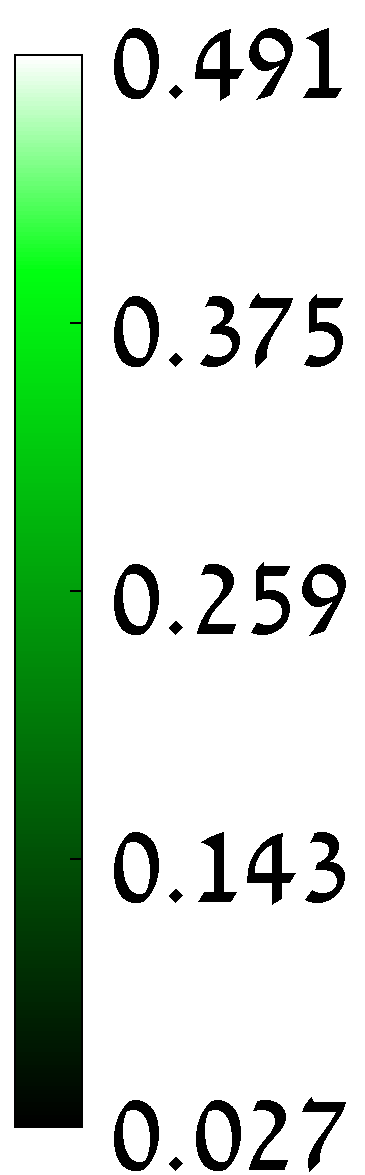
\includegraphics[height = 0.13\textwidth]{figs/confocal_res/fig_converging/4_BSI_fin_colorbar.pdf}&
			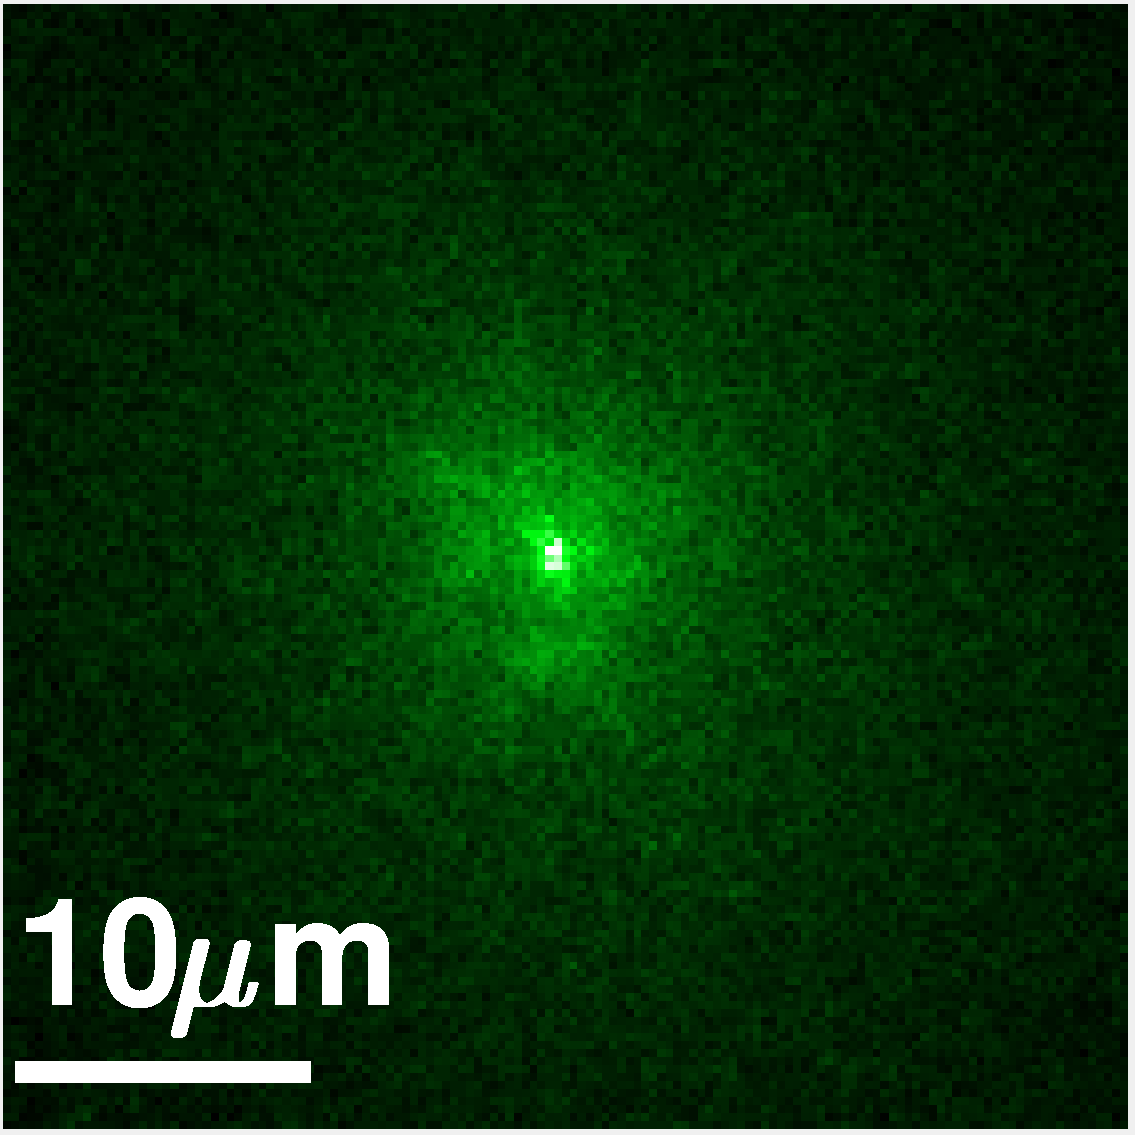
\includegraphics[height = 0.13\textwidth]{figs/confocal_res/fig_converging/4_BSI_fin_psf.pdf}&
			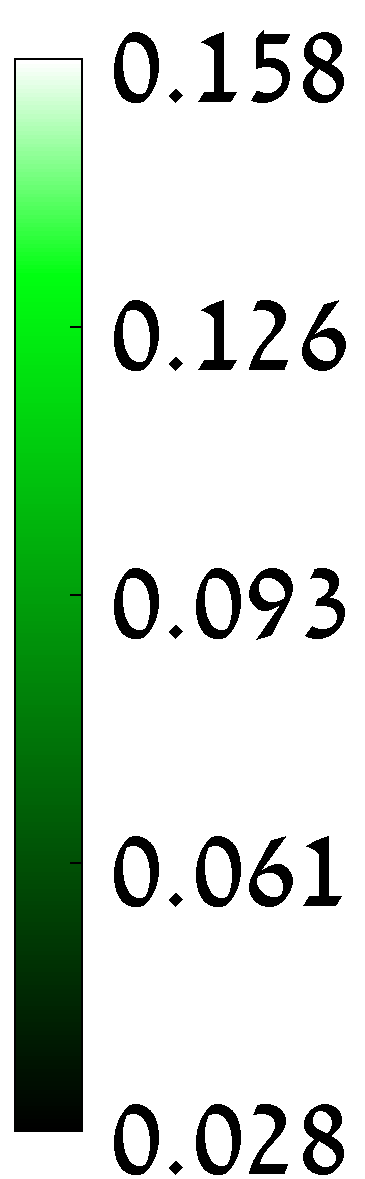
\includegraphics[height = 0.13\textwidth]{figs/confocal_res/fig_converging/4_BSI_fin_psf_colorbar.pdf}\\
					
			{\footnotesize{(a)  w/o mod.}} & {\footnotesize{ (b) w mod. }} & {\footnotesize{ (c) Reference}}  &     		
			\footnotesize{(d) w/o mod.} &   & \footnotesize{(e) w mod.} &   & \footnotesize{(f) PSF} \\
			\multicolumn{3}{c}{\footnotesize{Confocal scan of area}}&\multicolumn{6}{c}{\footnotesize{Single point}}
			
		\end{tabular}
		\caption{{\bf Wavefront shaping results:} Preliminary results of our 1P correction system imaging ex-vivo brain slices.  Left: Confocal scan of the neuron area.    (a) Image of the neuron with no correction, strong scattering is present and the neuron structure is lost. (b) Image with our modulation correction, the neuron shape as well as some of the axons are revealed. (c) A  reference  image of the same neuron. Right: To asses the amount of aberration we also present an image of a single  point. (d) While the objective attempts to focus at a single diffraction limited point, a wide speckle pattern is captured. (e) With modulation on both excitation and emission light we can observe a sharply focused spot. (f) To better asses aberration from one point, we correct only the incoming  light to focus and excite a single point, and measure the resulting scattered pattern
		}\label{fig:confocal-res}
	\end{center}
\end{figure*}



\subsubsection{Preliminary evaluation}
In \figref{fig:confocal-res}, we present preliminary results from~\cite{DrorNatureComm24}, where we utilized a confocal wavefront shaping system (correcting both emission and excitation) and a 1P laser to image EGFP neurons in ex-vivo slices of scattering brain tissue. Without correction, the neurons appear as wide, aberrated blobs. However, with our correction, the neuron shapes, including thin axons, are clearly revealed. The correction is valid through a limited spatial support but still one correction is sufficient for imaging the area around one neuron. 
To evaluate the actual aberration correction, the right part of \figref{fig:confocal-res} visualizes the image of a single point. By comparing \figref{fig:confocal-res}(d,e), we observe that our correction can increase the signal in the central pixel by a factor of  $\times4-\times 12$, depending on the amount of scattering present in the sample. This suggests that our goal of achieving a tenfold improvement in SNR is realistic.
In \figref{fig:confocal-res}(f), we use the modulation to excite a single point on the neuron and measure the resulting aberration without modulation in the emission arm. We find that the aberration has a compact support, making it feasible to correct different neurons with different SLM pixels.
\Anat{My main problem with the above results is that I have no clear documentation of the depth at which they were taken, and unfortently our setup is currently under construction and we will not be taking more measurments before the deadline... So all the numbers I gave in the aims part are just made up. On the other hand I am rather confident we can achieve at least a $\times 10$ improvment in SNR}

%\Anat{My main problem with the above results is that I have no clear documentation of the depth at which they were taken, and unfortently our setup is currently under construction and we will not be taking more measurments very soon. What I may mannage to do is take a few brain samples in different thicknesses and measure how much aberration we have, and see if it is comparable to the aberration we measured in  \figref{fig:confocal-res}(f). The following text is a place-holder, I hope I mannage to capture this before the deadline.}
%To estimate the number of aberration modes we need to correct, we imaged scattering through several brain slices. We focused a laser beam into a diffraction-limited spot on one side of the slice and captured the resulting speckles with a camera on the other side. \figref{} shows these speckle images, which exhibit limited support and thus can be corrected with a small number of SLM pixels.%Most of the aberrations targeted here are only a few dozen pixels wide.
%We also shifted the laser spot over a $10 \mu m$ square, corresponding to the typical size of a neuron. The speckle patterns are similar shifted versions of each other, indicating sufficient memory effect correlation. This suggests that all diffraction-limited spots on the same neuron can be corrected with the same SLM modulation.


\begin{figure*}[t!]
	\begin{center}
		\begin{tabular}{c}
		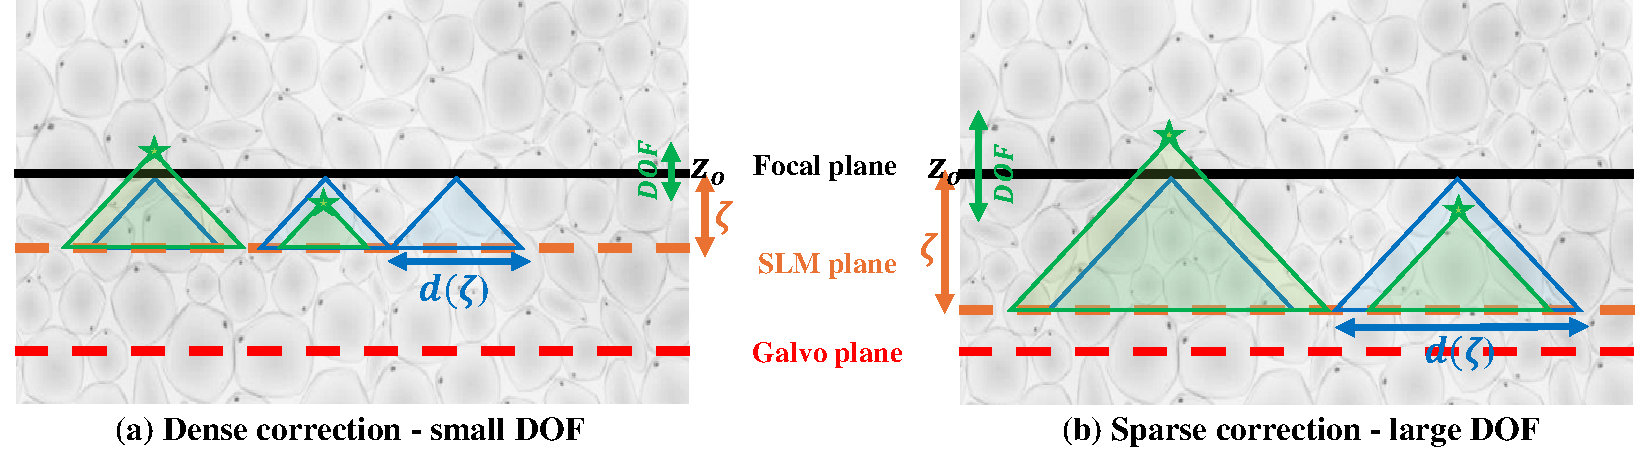
\includegraphics[width= 0.8\textwidth]{figs/system/DOF.pdf}
		%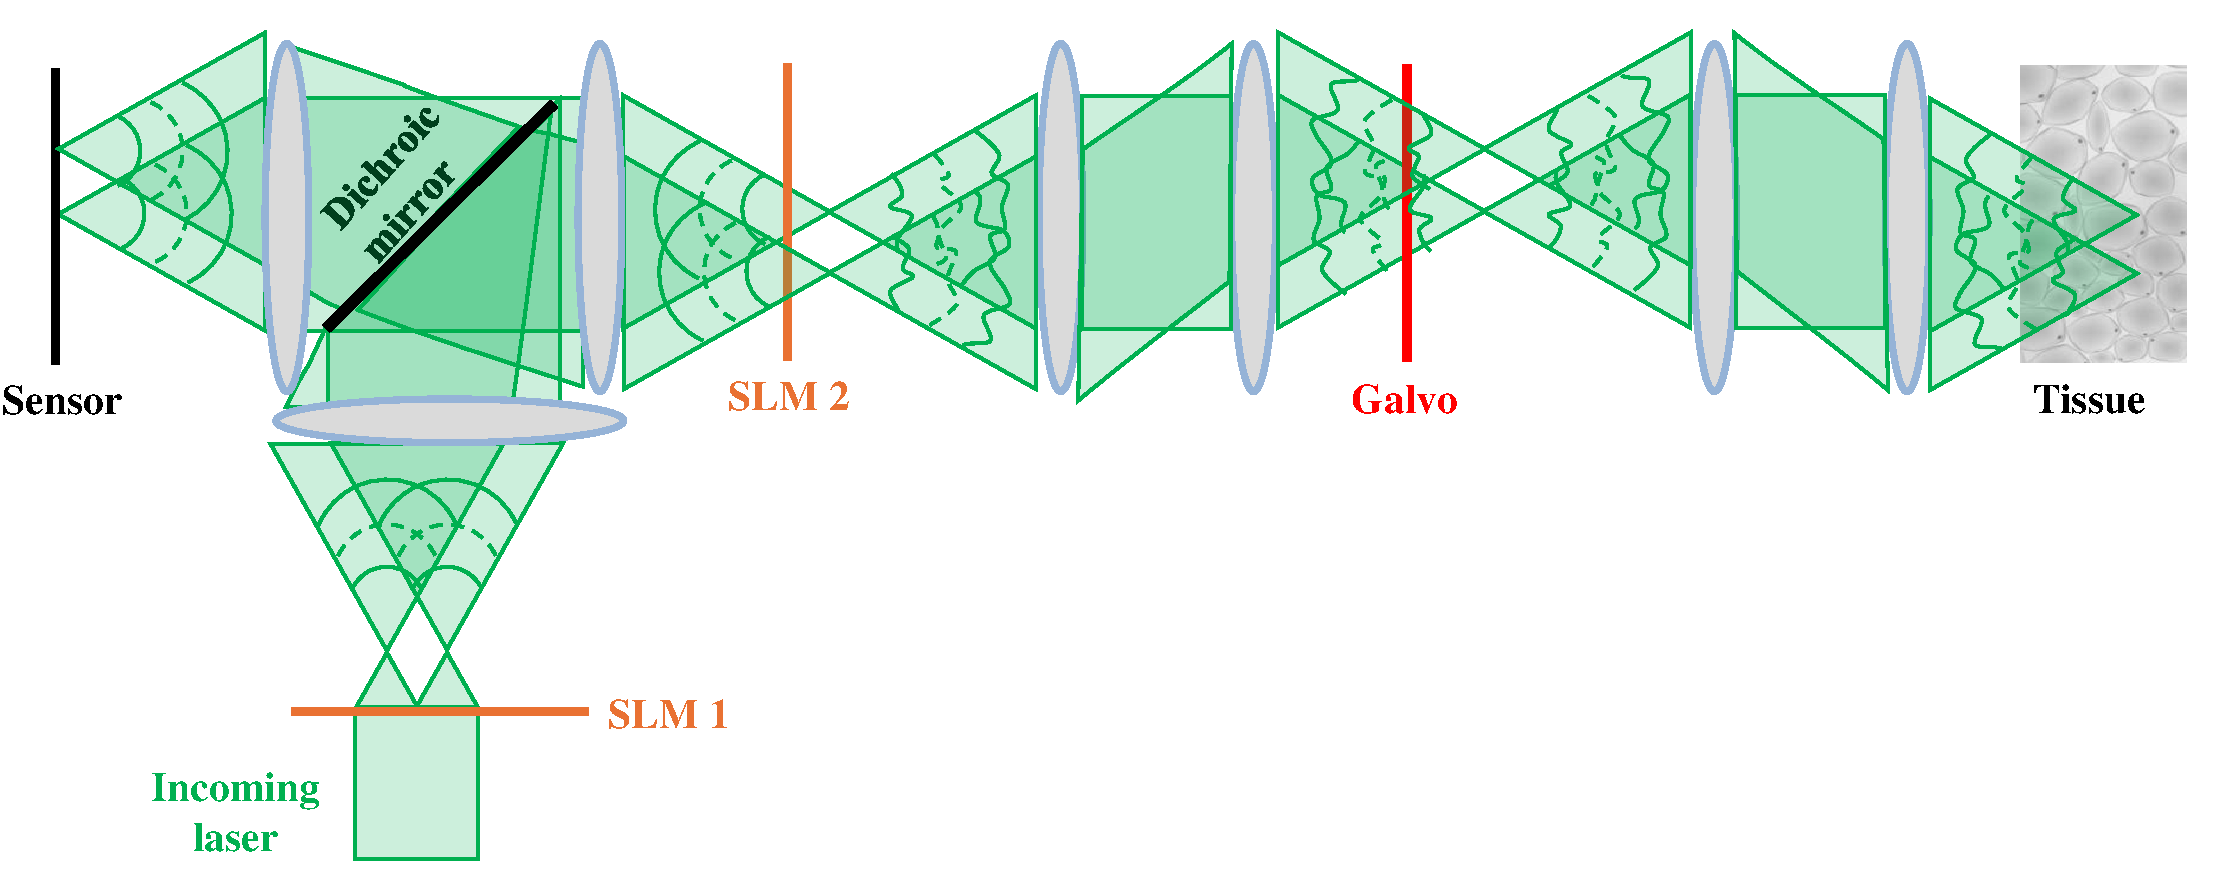
\includegraphics[width= 0.48\textwidth]{figs/system/oneP.pdf}\\
		%(a) Two photon&(b) One photon
		\end{tabular}
	\end{center}
	\caption{{\bf{Depth of field vs. sparsity:}} We visualize the conjugate position of the SLM modulation and the galvo tilt inside the brain tissue.  The distance of the SLM plane from the focal plane controls the diameter of defocus footprint from each target neuron. This diameter should be at least as large as the number of aberration modes one wish to correct. Increasing the distance allows more tolerance to depth variations of the target neurons, but as more SLM pixels are included in the footprint of each neuron, a sparser set of target neurons can be imaged. In the figure, blue triangles mark the idealized defocus blur of points on the focal point, and green triangles mark defocus footprint of sources at other depths.   } 

\label{fig:dof}
\end{figure*}


\subsubsection{Other considerations}\label{sec:otherconsiderations}
\boldstart{Target neural density and depth of field}
Our goal is to determine the number of neurons we can simultaneously correct with one SLM and the depth of field range in which they can be positioned. To understand this, consider \figref{fig:dof}. The camera sensor is conjugate to plane $z_o$ inside the volume, meaning that in the absence of tissue inhomogeneity, points at depth $z_o$ would be sharply focused on the sensor. The SLM is conjugate to a plane slightly before  $z_o$, at depth $z_o-\zeta$. 
To best utilize the SLM pixels, the system magnification is chosen such that a sensor pixel and an SLM pixel correspond to a diffraction limit unit  $\Delta=\lambda/(2NA)$ inside the tissue.
 
 In this setting, the value measured at each camera pixel is influenced by a disc of SLM pixels, corresponding to a defocus blur of diameter:
 \BE\label{eq:defocus-diameter}
 d(\zeta)=2 NA\cdot \zeta/\Delta.
 \EE  
 Clearly, for small  $\zeta$ values, the defocus blur is smaller, allowing us to  correct more neurons on the same SLM. On the other hand, the disc diameter should be at least as large as the number of aberration modes we wish to correct, ensuring we have enough degrees of freedom on our SLM. Moreover, if we use larger discs we can   tolerate a larger depth of field (DOF), meaning the target neurons do not have to be exactly at plane  $z_o$.
 Using a derivation that we omit due to space constraints, we conclude that if we aim to correct at least $50\%$ of the energy in the aberrated wavefront, by placing the SLM at distance $\zeta$, the depth range we can address corresponds to:
 \BE \label{eq:dof-slm-d} [z_o-0.3\zeta,z_o+0.4\zeta].\EE
 
 In the following table, we use \equpref{eq:defocus-diameter}{eq:dof-slm-d}  to test different depth-of-field targets and present a numerical evaluation of the number of different corrections we can fit on the SLM, namely the number of neurons we can correct. For the simulation, we assume 
  $NA=0.7$, $\lambda=510 nm$. % and that the aberration has a maximal support of $k \times k$ pixels with  $k=20$. 
We consider the recent Taxes Instrument SLM~\cite{PLM-TI_2019} with $800\times 1358$ pixels. 
\begin{center}
\begin{tabular}{|l|c|c|c|c|c|c|c|}
	\hline
	DOF [$\mu m$]&5&10&20&30&40&50&60\\\hline
	Defocus diameter [pixels]&28&56&112&   168 &  224&   280&   336\\
	Number of fitted corrections&1764 &        441 &        110  &        49 &         27 &         17  &        12 \\\hline
\end{tabular}
\end{center}
Most of the aberrations we target in this research are only a few dozen pixels wide, as shown in \figref{fig:confocal-res}(f) above. The table indicates that for a small DOF, where we can use compact support corrections, we can easily fit thousands of corrections on the SLM. Thought it is possible we will have to limit the number of target neurons to avoid too much background fluorescence. 
When using 2P excitation, we are likely limited to measuring 10-20 neurons due to power constraints~\cite{Davis2024Optical}. Given this limitation, there are enough pixels on the SLM to cover a DOF of nearly $50\mu m$.



 %While with 1P there is sufficient laser power to excite many neurons, the number of neurons we can address simultaneously is likely to be limited by background fluorescent, but hundreds of neurons can .  

% We note that when imaging a fluorescent spot inside the tissue, we achieve an aberrated speckle pattern. 
% However since the tissue is forward scattering and the brain depths we target here are modest this speckle pattern has a compact support. We present empirical examples of such speckle patterns in \figref{} above, most aberrations we target are a few dozen pixels wide. 
% In \figref{} we use \equref{eq:dof-slm-d} to present a numerical evaluation of the number of neurons we can correct as a function of depth of field. For the simulation we assume $NA=0.7$, $\lambda=0.5\mu m$ and that the aberration has a maximal support of $k \times k$ pixels with  $k=20$. 
%We consider the recent Taxes Instrument SLM~\cite{} with $800\times 1358$ pixels. 
%If we correct each neuron with only $20\times 20$ pixels we can easily fit on the SLM $2700$ different corrections. When trying to address a depth of field of $60\mu m$, the diameter of the needed correction increases to $285$ pixels and the number of different corrections we can fit decays to $15$. 
%When using 2P excitation we probably cannot measure more than 20 neurons due to power restrictions. With 1P we can address a much larger number of neurons but it is still likely that the number of neurons we can address is limited due to background fluorescence. 



%At the SLM plane the aberration corresponds to the convolution of the sensor aberration with a spherical wavefront $\rho_d$, corresponding to a propagation from plane $z_o$ to plane $z_o-d$,  so to correct the aberration we need to place on the SLM the conjugate of $u_\ptd\astr \rho_d$. 

\boldstart{Galvo tilting plane.} 
To achieve optimal memory effect correlation when scanning the wavefront shaping pattern over the neuron area, the SLM should ideally be placed at a plane conjugate to where the major aberration occurs~\cite{Mertz:15,Park2015,Tao2017}. Research~\cite{osnabrugge2017generalized,SeeThroughSubmission} suggests that this plane should be conjugate to $1/3\cdot z_o$,  where $z_o$
is the distance of the target neurons from the brain surface.
To accommodate different corrections on the SLM, we choose to place it much closer to the target plane. However, as noted by~\cite{Papadopoulos2020}, the SLM can be positioned anywhere in the optical path, provided the tilt occurs in a plane conjugate to the major aberration. Therefore, we design our system so that the galvo tilt plane is conjugate to a plane closer to the tissue surface, and the SLM plane is conjugate to a plane much closer to the actual target neurons, as illustrated in \figref{fig:dof}.

%Results in the literature states that to maximize 
%Our optical setup includes a galvo-mirror to allow fast scanning of a diffraction limited point over the neuron area. Previous research~\cite{osnabrugge2017generalized,SeeThroughSubmission} suggests that the ideal position for this tilt should be a plane conjugate to $1/3\cdot z_o$, where $z_o$ is the mean depth of target neurons from the brain surface, see \figref{fig:dof}.


\boldstart{Temporal stability.} \Anat{I think the question of speckle decorrelation time is the one that will draw most reviewer critisem. Any help in rewording the following text would be most valuable}
The current wavefront shaping system in PI Levin's lab is capable of estimating a wavefront shaping modulation in seconds. As part of this project we plan to incorporate machine learning techniques and develop algorithms that will further accelerate this estimation step.   After an initial modulation estimate stage, we can use the modulation to track neural activity, limited only by the camera frame rate. The SLM also allows us to tilt and direct the image of all neurons into a small subset of rows on the sensor, enabling us to read from the sensor at a 2 kHz frame rate.

An important concern is decorrelation time. For live tissue, we need to address blood flow, breathing, and other tissue dynamics, as well as the simple motion of the mouse. Since every sub-micron scale change in the length of the optical path can alter the speckle aberration, we may need to update our modulation frequently.
There have been numerous attempts to evaluate speckle decorrelation in the literature, measured under a wide range of experimental conditions, both in the context of diffused optical tomography~\cite{Durduran2010,berne2000dynamic,Boas:97,DynamicLightScattering}, and for wavefront shaping systems~\cite{Cui2010,Jang:15,Qureshi:17}. Most of these studies involved much thicker tissue samples than those we aim to handle in this project, so their conclusions may not directly apply to our case, because long diffused paths have a higher probability to cross blood vessels. 
% Diffused optical tomography~\cite{Durduran2010,berne2000dynamic,Boas:97,DynamicLightScattering} uses decorrelations on the order of milliseconds to infer blood flow and tissue structure. However, in such imaging systems, one measures very long light paths that have completely diffused and must pass through blood vessels.
%Several studies have measured speckle decorrelation for wavefront shaping~\cite{Cui2010,Jang:15,Qureshi:17}, with reported numbers varying significantly depending on experimental conditions. Most of these studies involved much thicker tissue samples than those we aim to handle in this project, so their conclusions may not directly apply to our case.
For the application scenarios considered in this research, the relevant light paths are mostly forward scattering, and we believe a sufficient percentage of such paths do not pass through blood vessels. For example, in~\cite{Yang2020Fighting}, the speckle decorrelation time of forward scattering paths was measured and analyzed. The authors observed that the part of the correlation associated with blood vessels decays rapidly in milliseconds. However, there is a second component of the signal, with about $60-70\%$ of its power, whose correlation holds for seconds and minutes. We believe that a wavefront shaping system that can utilize $60\%$ of the photons will already offer a significant improvement in SNR.
Similarly,\cite{Papadopoulos16} reported a wavefront shaping system applied for in-vivo 2P imaging, where the correction lasted for as long as 20 {\em minutes}. Additionally, studies in the literature explain that iterative wavefront shaping approaches effectively filter the dynamic part of the speckle and better adapt to the static component\cite{GU1994353,Blochet:19}.

Mice are usually well fixated under the microscope, and our prior experience is that they do not shift by more than a few microns. However, it is easy to track rigid motion and adjust the SLM pattern accordingly, as we did in previous research~\cite{Pegard2016Compressive}.\Anat{Is that the right citation?}  



\subsubsection{3D correction}
As analyzed in \secref{sec:otherconsiderations}, our SLM can tolerate a large depth of field with a sparse target neural population. If time permits, this research will also explore approaches to expand the depth range and density of neurons we can target simultaneously. One approach is to include a lenslet array and use a Fourier light field microscope~\cite{Pegard2016Compressive,Guo2019Fourier,Galdon2022Fourier}. However, capturing multiple viewpoints of the same neuron independently may reduce SNR.

An alternative approach is to use a multi-conjugate correction system with SLMs at multiple planes~\cite{Thaung:09,Wu:15,Laslandes:17,Furieri23,Kam2007,Simmonds_2013,Wu:15}. A third option follows~\cite{Xiao2018VideoRate} and involves scanning the volume with a very fast focus tunable lens synchronized with a fast DMD illuminating the target neural population. The DMD will illuminate each target neuron only when the focus tunable lens projects it at the desired target depth.


\subsection{Neurobiological approaches }
\Anat{Hillel, this part is yours}